\newpage
\section*{Exploration Questions}

\subsection*{Arc-length}
\begin{question}
	The parameterized curve
	\[
		\vec r(t) = \mat{2\cos t\\2\sin t}
	\]
	describes the position of a particle at time $t$.
	\begin{parts}
		\item Describe the path and motion of this particle in words.
		\item Compute the displacement  of the particle between $t=0$
			and $t=\Delta t$ and call the resulting vector $\Delta \vec r$.  
			(Assume $\Delta t$ is small.)
		\item Approximate the length of $\Delta \vec r$.  
			You may use the fact that
			when $x\approx 0$,
			\[
				\sin x\approx x\qquad\text{and}\qquad \cos x\approx -\tfrac{1}{2}x^2+1.
			\]
		\item Use a limit to compute the velocity of the particle at $t=0$. Call this 
			vector $\vec v_0$.
		\item Use a limit to compute the speed at $t=0$.  Call this value $s_0$.
		\item How do $\norm{\vec v_0}$ and $s_0$ relate?  Why?
	\end{parts}
\end{question}

\begin{question}
	A particle's path is parameterized by
	\[
		\vec m(t) = (f(t), g(t), h(t))
	\]
	where $t$ represents time.
	\begin{parts}
		\item Derive (with explanation) a formula for the velocity of
			the particle at time $t=t_0$.
		\item Derive (with explanation) a formula for the speed of
			the particle at time $t=t_0$.
	\end{parts}
\end{question}

\begin{question}
	Recall the particle whose path is given by
	$
		\vec r(t) = \mat{2\cos t\\2\sin t}
	$
	where $t$ represents time.
	\begin{parts}
		\item Use the fact that
			\[
				\text{distance traveled}=\int\text{\it speed}\ \mathrm{d}\,\text{\it time}
			\]
		to produce a formula for how far the particle has traveled from $t=0$ to $t=t_0$.
		\item Use geometry to do the same thing.
		\item Derive an expression (with explanation) for the arc length of $\vec m(t) = (f(t), g(t), h(t))$
			from $t=0$ to $t=t_0$.
	\end{parts}
\end{question}


\subsection*{Arc-length parameterization}
	An \emph{arc-length parameterization} of a curve $\mathcal C$ 
	is a function $\vec s:\R\to\R^n$ whose
	image is $\mathcal C$ with the added property that the arc 
	length of $\vec s(t)$ from $t=0$ to $t=t_0$
	is $t_0$ for all valid choices of $t_0$.  I.e., the distance 
	traveled by the parameter in
	$\R$ is the same as the distance traveled by the 
	point $\vec s(t)$ in $\R^n$.


\begin{question}
	\begin{parts}
		\item The function
			$
				\vec r(t) =\mat{2\cos t\\ 2\sin t}.
			$
			parameterizes a circle $\mathcal C$.  Produce an arc-length parameterization
			of $\mathcal C$.
		\item Produce an arc-length parameterization of the curve parameterized by
			$
				\vec q(t) =\mat{t\\ t^{3/2}}.
			$
	\end{parts}
\end{question}
	
	If you interpret a parameterized curve as describing the motion of a
	particle,
	an arc-length parameterization of a curve can also be thought of
	as a parameterization where the particle always moves at unit speed.

	By reparameterizing, we can describe the motion of a particle along
	a path at any speed.

\begin{question}
	Let $\mathcal C$ be a circle in $\R^2$ of radius $3$ centerd at the origin.
	A particle moves counter clockwise along $\mathcal C$.
	\begin{parts}
		\item Parameterize $\mathcal C$ so that the speed is $2.5$.
		\item Parameterize $\mathcal C$ so that the speed of the particle starts and ends at $0$.
		\item Parameterize $\mathcal C$ so that the speed of the particle starts at $0$ and ends at $4$.
		\item Parameterize $\mathcal C$ so that the speed of the particle is $0$ at six points along the curve.
	\end{parts}
\end{question}

\begin{question}
	A particle's motion is described by the function $\vec h(t) = \mat{f(t)\\ g(t)}$,  which is a 
	parameterization of the curve $\mathcal H$.  The arc length of $\mathcal H$ from $t=0$ to
	$t=t_0$ using this parameterization is given by the function $s(t_0) = t_0^2$.
	\begin{parts}
		\item Write an expression for the speed of the particle at time $t$.
		\item Give a formula for the arc length parameterization of $\mathcal H$.
	\end{parts}
\end{question}

\subsection*{Components of Acceleration}
\begin{restatable*}[Velocity]{definition}{DefVelocity}
	Let $\vec p:[a,b]\to\mathcal S$ be a parameterization of $\mathcal S$.  The
	\emph{velocity} of $\vec p$ at the time $t\in[a,b]$ is 
	\[
		\Vel \vec p(t) = \lim_{\Delta t\to 0} \frac{\vec p(t+\Delta t) - \vec p(t)}{\Delta t}.	
	\]
\end{restatable*}
\begin{restatable*}[Acceleration]{definition}{DefAcceleration}
	Let $\vec p:\R\to\mathcal S$ be a parameterization of $\mathcal S$.  The \emph{acceleration}
	of $\vec p$ is 
	\[
		\Accel \vec p(t) = (\Vel \vec p)'(t)=\vec p\,''(t).
	\]
\end{restatable*}

\begin{question}
	Let $\vec r(t) = \mat{t+2\\ \sin t\\ t^3}$ represent the position of a particle at time $t$.
	\begin{parts}
		\item Find the velocity of the particle at time $t$.
		\item Find the acceleration of the particle at time $t$.
	\end{parts}
\end{question}

\begin{question}
	Let $\vec r_\ell(t) = \mat{\frac{t^2}{2}\\\frac{t^2}{2}}$ and $\vec r_c(t) = \mat{\cos t\\ \sin t}$ give the position
	of the particles $r_\ell$ and $r_c$ at time $t$.
	\begin{parts}
		\item Describe the paths of each of these particles.  What should their accelerations be?  Why?
		\item Compute the accelerations of $r_\ell$ and $r_c$ at time $t$.
		\item Compute the tangent vectors for the functions $\vec r_\ell$ and $\vec r_c$ at time $t$.
			How does the direction of the tangent vectors and the direction of the acceleration vectors
			compare?
	\end{parts}
\end{question}

	If $\vec r(t)$ describes the position of a particle at time $t$ and $\vec a(t)$ its acceleration, $\vec a(t)$
	can be decomposed into a \emph{tangential} component, $\vec a_T(t)$, and a \emph{normal} component $\vec a_N(t)$
	so that
	\[
		\vec a(t) = \vec a_T(t) +\vec a_N(t).
	\]

\begin{question}
	Let $\vec r_{p}(t) = \mat{t\\ t^2}$ give the position
	of the particle $\vec r_{p}$ at time $t$.
	\begin{parts}
		\item Compute the tangential and normal components of the acceleration of $\vec r_{p}$.
		\item By changing the speed of $\vec r_{p}$ (but not its path), is it possible to make 
			the tangential component of its acceleration zero?
		\item By changing the speed of $\vec r_{p}$ (but not its path), is it possible to make 
			the normal component of its acceleration zero?
	\end{parts}
\end{question}

	We're going to develop some tools to mathematically verify our intuition about the acceleration
	vector.

\begin{question}
	\begin{parts}
		\item Suppose $\vec p(t)$ and $\vec q(t)$ are both vector-valued functions.  Expand $\vec p(t)\cdot\vec q(t)$
		using components. Now, come up with an expression for $\Big(\vec p(t)\cdot\vec q(t)\Big)'$.  Look at your
		result and rewrite it as an expression involving dot products.
		You've just discovered a product rule for the dot product!
		\item Using similar methods to the computation of $\Big(\vec p(t)\cdot\vec q(t)\Big)'$, find an expression
			for $\|\vec p(t)\|'$.
		\item If a particle whose path is given by $\vec r(t)$ is moving at unit speed, then $\|\vec v(t)\| = 1$.
			Take derivatives of both sides of this expression to show that $\vec v(t)\cdot \vec a(t) = 0$.
	\end{parts}

\end{question}


\newpage
\emph{Parameterization}\index{parameterization} is a mouthful, but the
fundamental idea of a parameterization is to describe one object in
terms of another.  For example, consider the line $\ell$ described
by the equation $y=2x$.  By its nature, $\ell$ is a set.
Using set-builder notation, we could write
\[
	\ell = \Set*{\mat{x\\y}\given y=2x}.
\]
But, we could also write $\ell$ in vector form as 
\[
	\mat{x\\y}=t\mat{1\\2}.
\]
Writing $\ell$ in vector form shows a pairing between scalars $t\in \R$
and points on $\ell$.  In many ways, $\ell$ is the same as $\R$---it's
just sitting in two-dimensional space instead of being on its own.

Taking a more technical viewpoint, we may consider $\ell$ to be the range of 
a vector-valued function.  Define $\vec p(t) = t\mat{1\\2}$.  Then,
\[
	\ell = \Range(\vec p) = \Set*{\vec x\given \vec x=\vec p(t)\text{ for some }t\in\R}.
\]
Now we have something special.  The function $\vec p:\R\to\R^2$ has domain $\R$ and outputs
every point on the line $\ell$ exactly once.  In other words, we've described
$\ell$ in terms of $\R$ and $\vec p$.  We could make a further assertion
that \emph{anything that you could learn by studying $\ell$, you could learn
by studying $\R$ and $\vec p$}.

However, there are other ways to create functions that describe $\ell$.
For example, consider $\vec q:\R\to\R^2$ where $\vec q(t)=2t\vec d$.  Again,
$\ell = \Range(\vec q)$ and so everything we could possibly learn about
$\ell$, we could learn by studying $\R$ and $\vec q$.
We call both $\vec p$ and $\vec q$ \emph{parameterizations of $\ell$ by $\R$}.

\begin{definition}[Parameterization]
	A \emph{parameterization} of an object $X$ by an object $Y$ is a continuous
	function $p:Y\to X$ with the added conditions that $p$ is one-to-one\footnote{
	Sometimes we will drop the requirement that a parameterization be one-to-one,
	but for now we'll be strict about it.}
	and $\Range(p)= Y$.  In this case $p$ is called a \emph{parameterization} and $Y$ is
	called the \emph{parameter}.
\end{definition}

This definition is fairly abstract, which will come in handy later. For
now, we will think of $X$ as being some curve in $\R^n$ and $Y$ as being an
interval of real numbers.

\begin{example}[A Circle]
	Let $\mathcal C\subseteq \R^2$ be the unit circle centered at the origin.
	We can parameterize $\mathcal C$ by angles in $[0,2\pi)$.  Consider the function
	$\vec p:[0,2\pi)\to\mathcal C$ defined by
	\[
		\vec p(\theta) = \mat{\cos\theta \\\sin \theta}.	
	\]
	Here, $\vec p$ traces out $\mathcal C$ starting at the point $(1,0)$ and
	moving counter clockwise as the parameter $\theta$ increases.
\end{example}
\begin{example}[A Circle Again]
	Let $\mathcal C\subseteq \R^2$ be the unit circle centered at the origin.
	We will parameterize $\mathcal C$ by the interval $[0,1)$.  Here we might
	imagine that our parameter $t\in[0,1)$ represents a point that is $t$-percentage
	around the circle.  
	
	Recall $\vec p(\theta)=\mat{\cos \theta\\\sin\theta}$, which parameterizes
	$\mathcal C$ based on angles.
	
	Now, consider the function $w(t) =2\pi t$.
	$w$ inputs numbers in $[0,1)$ and outputs angles in $[0,2\pi)$.  We should
	now be able to use $w$ to parameterize $\mathcal C$ in the desired way.
	After all, if we convert $[0,1)$ to $[0,2\pi)$ to $\mathcal C$, we win!

	Let the parameterization
		$\vec q:[0,1)\to\mathcal C$ be defined as $\vec q=\vec p\circ w$.
	Explicitly,
	\[
		\vec q(t) = \vec p\circ w(t) = \vec p(2\pi t) = \mat{\sin 2\pi t\\\cos 2\pi t}.	
	\]
\end{example}

\begin{exercise}
	Parameterize the unit circle $\mathcal C\subseteq \R^2$ by the interval $[1/2,1)$.
\end{exercise}
\begin{exercise}
	Let $\ell$ be the line segment connecting $(0,0)$ and $(1,1)$.
	Explain why $\vec p:[-1,1]\to\ell$ given by $p(t)=(t^2,t^2)$ is \emph{not}
	a parameterization.
\end{exercise}

\section{Speed and Velocity of a Parameterization}

In our day-to-day life, almost without thinking, we make a comparison between real numbers
and time.  Time has a forwards and backwards, which we equate to
the real number's increasing and decreasing.  We might even say we parameterize \emph{time}
by the real numbers.  Thus, if $\vec p:[a,b]\to \mathcal S$ is a parameterization 
of the curve $\mathcal S$ by the interval $[a,b]$, we could think of $\vec p$ as describing
the motion of a particle---at time $t\in[a,b]$ the particle is at $\vec p(t)$.

Interpreting parameterizations in this way, the \emph{speed}\index{speed} of a parameterization
should be the rate of change of distance with respect to time and the \emph{velocity}\index{velocity}
of a parameterization should be the rate of change of displacement with respect to time.

Suppose $\vec p:[a,b]\to\mathcal S$ is a parameterization of $\mathcal S$ and $t\in[a,b]$
represents time.  The \emph{displacement} of $\vec p$ from time $t$ to time $t+\Delta t$ is
$\vec p(t+\Delta t)-\vec p(t)$ and the change in \emph{distance} is $\norm{\vec p(t+\Delta t) - \vec p(t)}$.
Thus, if $\Delta t$ is small, the velocity at time $t$ can be approximated by
\[
		\Vel \vec p(t) \approx \frac{\vec p(t+\Delta t) - \vec p(t)}{\Delta t}	
\]
and the speed\footnote{
		Recall that speed is always positive; if a particle is moving with speed $2$
		and we then ran the particle back in time, it would still move at speed $2$,
		so speed is not $\text{distance}/\Delta t$, it is $\text{distance}/\abs{\Delta t}$.
		} by
\[
	\Speed \vec p(t) \approx \frac{\norm{\vec p(t+\Delta t) - \vec p(t)}}{\abs{\Delta t}}.	
\]
Taking limits, we arrive at exact rates of change, which leads us to the following definitions.
\begin{definition}[Speed]
	Let $\vec p:[a,b]\to\mathcal S$ be a parameterization of $\mathcal S$.  The
	\emph{speed} of $\vec p$ at the time $t\in[a,b]$ is 
	\[
		\Speed \vec p(t) = \lim_{\Delta t\to 0} \frac{\norm{\vec p(t+\Delta t) - \vec p(t)}}{\abs{\Delta t}}.	
	\]
\end{definition}
\DefVelocity

Both the definition of speed and the definition of velocity look a lot like the definition
of the derivative.  In fact, if $\vec p$ were a scalar valued function, the velocity of $\vec p$
would be exactly the derivative of $\vec p$.  For this reason, we will define a notation
similar to that of the derivative you're familiar with.  From now on, the following notations mean
the same thing:
\[
	\Vel \vec p(t) = \vec p\,'(t) = \frac{\d}{\d t}\vec p(t) = \frac{\d \vec p}{\d t}(t).
\]

Let's try to use our new definition.  Let $\vec r(t) = \mat{\cos t\\\sin t}$.  Now,
\begin{align*}
	\Vel \vec r(t) &=\lim_{\Delta t\to 0} \frac{\mat{\cos(t+\Delta t)\\\sin(t+\Delta t)} - \mat{\cos t\\\sin t}}{\Delta t}\\
	&=\lim_{\Delta t\to 0} \mat{
		\displaystyle\frac{\cos(t+\Delta t)-\cos t}{\Delta t} \\\displaystyle\frac{\sin(t+\Delta t)-\sin t}{\Delta t}
		}.
\end{align*}
At this point, we should pause.  We don't know how to take limits of vectors.  Fortunately the rule
is simple enough---to take a limit of a vector, take the limit of each of its components\footnote{
	As intuitive as it sounds, this rule actually has a proof which relies on the definition
	of limit and the continuity of $\norm{\:\cdot\:}$.
}.  Thus we see
\begin{align*}
	\Vel \vec r(t) 
	&=\lim_{\Delta t\to 0} \mat{
		\displaystyle\frac{\cos(t+\Delta t)-\cos t}{\Delta t} \\\frac{\displaystyle\sin(t+\Delta t)-\sin t}{\Delta t}}\\
	&=\mat{
		\displaystyle\lim_{\Delta t\to 0} \frac{\cos(t+\Delta t)-\cos t}{\Delta t} \\\displaystyle\lim_{\Delta t\to 0} \frac{\sin(t+\Delta t)-\sin t}{\Delta t}
		}\\
	&=\mat{\cos'(t)\\\sin'(t)} = \mat{-\sin t\\\cos t}.
\end{align*}
Our use of the notation $\vec r\,'(t)$ for $\Vel \vec r(t)$ seems further justified.

Speed also appears to be a derivative.  From physics, we know that speed is the magnitude of 
velocity.  We can prove it mathematically.
\begin{theorem}
	For a parameterization $\vec p:\R\to\R^n$ where $\Vel \vec p(t)$
	exists, we have
	\[
		\Speed \vec p(t) = \norm{\Vel \vec p(t)} = \norm{\vec p\,'(t)}.
	\]
\end{theorem}
\begin{proof}
	The proof relies on the continuity of $\norm{\:\cdot\:}$.  Since $\norm{\:\cdot\:}$
	is continuous, we may freely move limits in and out\footnote{
		This limit rule actually says if $f$ is continuous 
		\emph{and} $\lim_{x\to a} g(x)$ exists, then $\lim_{x\to a}f(g(x))
		=f\big(\lim_{x\to a}g(x)\big)$.}.  Thus
	\begin{align*}
		\Speed \vec p(t) &= \lim_{\Delta t\to 0} \frac{\norm{\vec p(t+\Delta t) - \vec p(t)}}{\abs{\Delta t}}\\
		&= \lim_{\Delta t\to 0} \norm*{\frac{\vec p(t+\Delta t) - \vec p(t)}{\Delta t}}\\
		&=\norm*{\lim_{\Delta t\to 0} \frac{\vec p(t+\Delta t) - \vec p(t)}{\Delta t}}
		=\norm{\Vel \vec p(t)}.
	\end{align*}
\end{proof}

\subsection{Arc-length}
Let $\mathcal S\subseteq \R^n$ be a curve parameterized by $\vec p:[a,b]\to\R^n$.  
The \emph{arc-length}\index{arc length} of $\mathcal S$
should be the length of $\mathcal S$ if you somehow untwisted $\mathcal S$ into a straight
line without stretching anything.  One of the big ideas of calculus is that 
we can handle curvy things by chopping them up into little pieces, computing
for each piece, and then adding them back together.  We use the same principle 
to define arc-length.

In essence, we will divide our curve $\mathcal S$ into many tiny line segments,
add up the lengths of those line segments and take a limit as our line segments
get tinier.  A parameterization provides us with a way to do this.  Since parameterizations
are continuous, if we chop the domain of the parameterization into tiny pieces,
we will have chopped the range into tiny pieces.


% Some nice looking curves:
% x=sin(t^.7)*(t/4-t^2/30)*10+2
% y=((10-t)^.5+t^2/10)*cos(t/10)
% [0,10]
%
% or
% x=-(t+1)*t*(t-3)*(1+t^2)/4
% y=-t*(t-1)*(t-2)*4*(1+t^3)/4
% [0,2]

\begin{center}
	\begin{tikzpicture}
		\begin{axis}[
		    name=plot1,
		    %anchor=origin,
		    %disabledatascaling,
		    xmin=-1,xmax=8,
		    ymin=-1,ymax=2.5,
		    x=1cm,y=1cm,
		    xtick=\empty,ytick=\empty,
		    grid=both,
		    grid style={line width=.1pt, draw=gray!10},
		    %major grid style={line width=.2pt,draw=gray!50},
		    axis lines=middle,
		    minor tick num=0,
		    enlargelimits={abs=0.5},
		    axis line style={latex-latex},
		    ticklabel style={font=\tiny,fill=white},
		    xlabel style={at={(ticklabel* cs:1)},anchor=north west},
		    ylabel style={at={(ticklabel* cs:1)},anchor=south west}
		]

		\addplot[domain=0:2, samples=80, thick, mypink] ({-(x+1)*x*(x-3)*(1+x^2)/4},{-x*(x-1)*(x-2)*4*(1+x^3)/4});
		\addplot[domain=0:2, samples=15, only marks, mark=|, gray, thick] ({-(x+1)*x*(x-3)*(1+x^2)/4},{-x*(x-1)*(x-2)*4*(1+x^3)/4});
		\addplot[domain=0:2, samples=15, gray,thick] ({-(x+1)*x*(x-3)*(1+x^2)/4},{-x*(x-1)*(x-2)*4*(1+x^3)/4});
		\draw[] (0,2.5) node[right,gray] {Approximation by Line Segments};
		\draw[] (0,.5) node[right] {Range};

		\end{axis}
		\begin{axis}[
		    at=(plot1.below south),anchor=above north,yshift=-.5cm,
		    %anchor=origin,
		    %disabledatascaling,
		    xmin=-1,xmax=8,
		    ymin=-.2,ymax=.2,
		    hide y axis,
			xtick=\empty,
		    x=1cm,y=1cm,
		    grid=both,
		    grid style={line width=.1pt, draw=gray!10},
		    %major grid style={line width=.2pt,draw=gray!50},
		    axis lines=middle,
		    minor tick num=0,
		    enlargelimits={abs=0.5},
		    axis line style={latex-latex},
		    ticklabel style={font=\tiny,fill=white},
		    xlabel style={at={(ticklabel* cs:1)},anchor=north west},
		    ylabel style={at={(ticklabel* cs:1)},anchor=south west}
		]

			\addplot[domain=0:6, samples=2, thick, mypink] ({x},{0});
		\addplot[domain=0:6, samples=15, only marks, mark=|, gray, thick] ({x},{0});
		\draw[] (0,.5) node[right] {Domain};

		\end{axis}
	\end{tikzpicture}
\end{center}

To find the arc-length of a curve, we will approximate each tiny piece with a straight
line segment connecting the endpoints.  We then add up the lengths of all tiny segments
and take a limit as our segment's length goes to zero.

\begin{definition}[Arc-length]
	Let $\mathcal S\subseteq \R^n$ be a curve parameterized by $\vec p:[a,b]\to\mathcal S$. 
	The \emph{arc-length}
	of $\mathcal S$ is 
	\[
		\Arclen\mathcal S = \lim_{\Delta t\to 0^+} \sum_{i=1}^{\frac{b-a}{\Delta t}} 
		\,\norm{\vec p(a+(i-1)\Delta t)-\vec p(a+i\Delta t)}.
	\]
\end{definition}

There's something unsatisfying about this definition, though.  We used a parameterization
of $\mathcal S$ to compute the arc-length of $\mathcal S$.  But $\mathcal S\subseteq \R^n$ 
is a curve regardless of whether or not it has a parameterization, and if you use a different
parameterization, you should get the same arc length for $\mathcal S$.  If you're worried about
this, good!  You're thinking carefully!  We won't show it here, but in fact no matter what parameterization
you use for a curve, this definition will always produce the same arc length.

There's another reason we might be unhappy with this definition.  Limits of sums are
hard to compute!  However, the sum involved in arc-length looks very close to a Riemann sum.
If we can rewrite it exactly as a Riemann sum, we can replace it with an integral.  With some
superficial manipulation we see

\begin{align*}
	\Arclen\mathcal S 
	&= \lim_{\Delta t\to 0^+} \sum_{i=1}^{\frac{b-a}{\Delta t}} 
	\,\norm{\vec p(a+(i-1)\Delta t)-\vec p(a+i\Delta t)}\\
	&= \lim_{\Delta t\to 0^+} \sum_{i=1}^{\frac{b-a}{\Delta t}} 
	\,\frac{\norm{\vec p(a+(i-1)\Delta t)-\vec p(a+i\Delta t)}}{\Delta t}\Delta t\\
	&=\int_{a}^b \Speed \vec p(t)\,\d t.
\end{align*}

For the last equality, we noticed that 
$\lim_{\Delta t\to 0^+} \frac{\norm{\vec p(t)-\vec p(t+\Delta t)}}{\Delta t}=\Speed \vec p(t)$,
which involved switching a limit and an infinite sum.  In order to do this rigorously, we need
a mathematical proof that it is logically valid.  Such a proof is the subject of a course in
\emph{real analysis}, and won't be covered here, but it's always good to keep track of what
you've actually proved and what you've been told is true\footnote{ In order to prove that swapping
the limit and sum is valid, we actually need extra assumptions on $\vec p$.  If we make $\vec p$
\emph{differentiable} rather than merely \emph{continuous}, we can prove that the swap is valid.}.

Speed is easy to calculate, and we have a better handle on calculating integrals than we do 
limits of sums, so now we have a chance of calculating arc-length.

\begin{example}
	\label{EXHARDARCLEN}
We shall find the length of the parabola with equation $y = x^2$
on the interval $-1\le x \le 1$.   A parametric representation
	of the parabola is $\vec p(t) = (t,t^2)$
where $-1 \le t \le 1$.  
Now,
\[
	\frac{\d\vec p}{\d t} = \mat{1\\2t},
\]
so $\Speed \vec p(t)=\norm{\vec p\,'(t)} = \sqrt{ 1 + 4t^2}$.
Hence,
\[
  L = \int_{-1}^1 \sqrt{1 + 4t^2} dt = \sqrt 5 + 
\frac 14\ln\frac{\sqrt 5 + 2}{\sqrt 5 - 2}.
\]
\end{example}

As you can see from Example \ref{EXHARDARCLEN}, the integrals involved in computing
arc length can be difficult.  In fact, most of them don't have an elementary form, which
means in the real world we often use a computer to approximate arc length directly from the Riemann sum
rather than calculate it exactly.

\begin{exercises}
\end{exercises}

\section{Arc-length Parameterization}

Recall a parameterization is a relation between two objects.  If a curve $\mathcal S\subseteq\R^n$
is parameterized by $\R$, it means there is a continuous, one-to-one function $\vec p:\R\to\mathcal S$.
This function can be thought of as a map from $\R$ to $\mathcal S$.  Any interval $[a,b]\subseteq\R$
corresponds to a segment $\vec p([a,b])\subseteq \mathcal S$.

\begin{center}
	\usetikzlibrary{patterns,decorations.pathreplacing}
	\begin{tikzpicture}
		\begin{axis}[
		    name=plot1,
		    %anchor=origin,
		    %disabledatascaling,
		    xmin=-1,xmax=8,
		    ymin=-1,ymax=2.5,
		    x=1cm,y=1cm,
		    xtick=\empty,ytick=\empty,
		    grid=both,
		    grid style={line width=.1pt, draw=gray!10},
		    %major grid style={line width=.2pt,draw=gray!50},
		    axis lines=middle,
		    minor tick num=0,
		    enlargelimits={abs=0.5},
		    axis line style={latex-latex},
		    ticklabel style={font=\tiny,fill=white},
		    xlabel style={at={(ticklabel* cs:1)},anchor=north west},
		    ylabel style={at={(ticklabel* cs:1)},anchor=south west}
		]
		
		\pgfmathsetmacro\mystart{1.2}
		\pgfmathsetmacro\myend{1.7}
		\coordinate (A) at ($({-(\mystart+1)*\mystart*(\mystart-3)*(1+\mystart^2)/4},{-\mystart*(\mystart-1)*(\mystart-2)*4*(1+\mystart^3)/4})$);
		\coordinate (B) at ($({-(\myend+1)*\myend*(\myend-3)*(1+\myend^2)/4},{-\myend*(\myend-1)*(\myend-2)*4*(1+\myend^3)/4})$);

		\addplot[domain=0:2, samples=80, thick, mypink] ({-(x+1)*x*(x-3)*(1+x^2)/4},{-x*(x-1)*(x-2)*4*(1+x^3)/4});
		\addplot[domain=\mystart:\myend, samples=20, ultra thick, blue] ({-(x+1)*x*(x-3)*(1+x^2)/4},{-x*(x-1)*(x-2)*4*(1+x^3)/4});
		\draw[] (0,.5) node[right] {Range};
		
		\draw[fill] (A) circle (1.5pt) node[above left] {$\vec p(a)$};
		\draw[fill] (B) circle (1.5pt) node[above] {$\vec p(b)$};

		\end{axis}
		\begin{axis}[
		    at=(plot1.below south),anchor=above north,yshift=-.5cm,
		    %anchor=origin,
		    %disabledatascaling,
		    xmin=-1,xmax=8,
		    ymin=-.2,ymax=.2,
		    hide y axis,
			xtick=\empty,
		    x=1cm,y=1cm,
		    grid=both,
		    grid style={line width=.1pt, draw=gray!10},
		    %major grid style={line width=.2pt,draw=gray!50},
		    axis lines=middle,
		    minor tick num=0,
		    enlargelimits={abs=0.5},
		    axis line style={latex-latex},
		    ticklabel style={font=\tiny,fill=white},
		    xlabel style={at={(ticklabel* cs:1)},anchor=north west},
		    ylabel style={at={(ticklabel* cs:1)},anchor=south west}
		]

		\addplot[domain=0:6, samples=2, thick, mypink] ({x},{0});
		\draw[] (0,.5) node[right] {Domain};
		\coordinate (A) at (3,0);
		\coordinate (B) at (5,0);
		\draw[ultra thick, blue] (A) -- (B);
		\draw[fill] (A) circle (1.5pt)  node[above] {$a$};
		\draw[fill] (B) circle (1.5pt)  node[above] {$b$};

		\end{axis}
	\end{tikzpicture}
\end{center}

Alternatively, we may think of $\vec p:\R\to\mathcal S$ as a function that picks up the real line,
stretches, twists, and warps it, and sticks it into $\R^n$ in the shape of $\mathcal S$.
In this sense, not all parameterizations are created equally.  Some significantly stretch and warp
and others barely do at all.  

\begin{center}
	\usetikzlibrary{patterns,decorations.pathreplacing}
	\begin{tikzpicture}
	\pgfmathsetmacro{\samplestep}{4}
		\begin{axis}[
		    name=plot1,
		    %anchor=origin,
		    %disabledatascaling,
		    xmin=-1,xmax=8,
		    ymin=-1,ymax=2.5,
		    x=1cm,y=1cm,
		    xtick=\empty,ytick=\empty,
		    grid=both,
		    grid style={line width=.1pt, draw=gray!10},
		    %major grid style={line width=.2pt,draw=gray!50},
		    axis lines=middle,
		    minor tick num=0,
		    enlargelimits={abs=0.5},
		    axis line style={latex-latex},
		    ticklabel style={font=\tiny,fill=white},
		    xlabel style={at={(ticklabel* cs:1)},anchor=north west},
		    ylabel style={at={(ticklabel* cs:1)},anchor=south west}
		]

		\draw[] (0,.5) node[right] {Range};
		

			\addplot[domain=0:2, samples=80, ultra thick, myorange,
			    x filter/.code={%
				\pgfmathsetmacro{\orig}{\pgfmathresult}
				\pgfmathsetmacro{\modcoord}{mod(int(mod(\coordindex, 2*\samplestep)),2*\samplestep)}
				\pgfmathparse{\modcoord <= \samplestep ? \orig : nan}
			    }, unbounded coords=jump] ({-(x+1)*x*(x-3)*(1+x^2)/4},{-x*(x-1)*(x-2)*4*(1+x^3)/4});
			\addplot[domain=0:2, samples=80, ultra thick, blue,
			    x filter/.code={%
				\pgfmathsetmacro{\orig}{\pgfmathresult}
				\pgfmathsetmacro{\modcoord}{mod(int(mod(\coordindex, 2*\samplestep)),2*\samplestep)}
				\pgfmathparse{\modcoord == 0 || \modcoord >= \samplestep ? \orig : nan}
			    }, unbounded coords=jump] ({-(x+1)*x*(x-3)*(1+x^2)/4},{-x*(x-1)*(x-2)*4*(1+x^3)/4});
		\end{axis}
		\begin{axis}[
		    at=(plot1.below south),anchor=above north,yshift=-.5cm,
		    %anchor=origin,
		    %disabledatascaling,
		    xmin=-1,xmax=8,
		    ymin=-.2,ymax=.2,
		    hide y axis,
			xtick=\empty,
		    x=1cm,y=1cm,
		    grid=both,
		    grid style={line width=.1pt, draw=gray!10},
		    %major grid style={line width=.2pt,draw=gray!50},
		    axis lines=middle,
		    minor tick num=0,
		    enlargelimits={abs=0.5},
		    axis line style={latex-latex},
		    ticklabel style={font=\tiny,fill=white},
		    xlabel style={at={(ticklabel* cs:1)},anchor=north west},
		    ylabel style={at={(ticklabel* cs:1)},anchor=south west}
		]
			\addplot[domain=0:6, samples=81, ultra thick, myorange,
			    x filter/.code={%
				\pgfmathsetmacro{\orig}{\pgfmathresult}
				\pgfmathsetmacro{\modcoord}{mod(int(mod(\coordindex, 2*\samplestep)),2*\samplestep)}
				\pgfmathparse{\modcoord <= \samplestep ? \orig : nan}
			    }, unbounded coords=jump] ({x},{0});
			\addplot[domain=0:6, samples=81, ultra thick, blue,
			    x filter/.code={%
				\pgfmathsetmacro{\orig}{\pgfmathresult}
				\pgfmathsetmacro{\modcoord}{mod(int(mod(\coordindex, 2*\samplestep)),2*\samplestep)}
				\pgfmathparse{\modcoord == 0 || \modcoord >= \samplestep ? \orig : nan}
			    }, unbounded coords=jump] ({x},{0});

		\draw[] (0,.5) node[right] {Domain};

		\end{axis}
	\end{tikzpicture}
\end{center}


The least stretchy type of parameterization is called an \emph{arc-length
parameterization}\index{arc-length parameterization}.

Before we define arc-length parameterization, let's introduce some notation.  If $\mathcal S\subseteq \R^n$
is a curve parameterized by $\vec p:\R\to\mathcal S$, then
\[
	\Arclenfrom{\vec p}{a}{b}  = \text{ arc length of $\mathcal S$ between $\vec p(a)$ and $\vec p(b)$}.
\]
We might read $\Arclenfrom{\vec p}{a}{b}$ as the ``arc length of the curve traced by $\vec p(t)$ from
$t=a$ to $t=b$.''  Using notion for the \emph{image} of a set, we can also write
\[
	\Arclenfrom{\vec p}{a}{b} = \Arclen \vec p([a,b]).
\]

\begin{definition}
	Let $\mathcal S\subseteq\R^n$ be a curve and $\vec p:\R\to\mathcal S$ be a parameterization.
	The parameterization $\vec p$ is called an \emph{arc-length parameterization} if for $b\geq a$,
	\[
		\Arclenfrom{\vec p}{a}{b}=b-a.
	\]
\end{definition}

In plain language, if $\vec p$ is an arc-length parameterization, then the distance traveled in parameter
space is the same as the distance traveled along the curve.

\begin{center}
	\usetikzlibrary{patterns,decorations.pathreplacing}
	\begin{tikzpicture}
	\pgfmathsetmacro{\samplestep}{4}
		\begin{axis}[
		    name=plot1,
		    %anchor=origin,
		    %disabledatascaling,
		    xmin=-1,xmax=8,
		    ymin=-1,ymax=2.5,
		    x=1cm,y=1cm,
		    xtick=\empty,ytick=\empty,
		    grid=both,
		    grid style={line width=.1pt, draw=gray!10},
		    %major grid style={line width=.2pt,draw=gray!50},
		    axis lines=middle,
		    minor tick num=0,
		    enlargelimits={abs=0.5},
		    axis line style={latex-latex},
		    ticklabel style={font=\tiny,fill=white},
		    xlabel style={at={(ticklabel* cs:1)},anchor=north west},
		    ylabel style={at={(ticklabel* cs:1)},anchor=south west}
		]

		\draw[] (0,.5) node[right] {Range};
		

			\addplot[domain=0:2, samples=80, ultra thick, myorange,
				dash pattern=on 8pt off 8pt
			    ] ({-(x+1)*x*(x-3)*(1+x^2)/4},{-x*(x-1)*(x-2)*4*(1+x^3)/4});
			\addplot[domain=0:2, samples=80, ultra thick, blue,
				dash pattern=on 8pt off 8pt, dash phase=8pt
			    ] ({-(x+1)*x*(x-3)*(1+x^2)/4},{-x*(x-1)*(x-2)*4*(1+x^3)/4});
		\end{axis}
		\begin{axis}[
		    at=(plot1.below south),anchor=above north,yshift=-.5cm,
		    %anchor=origin,
		    %disabledatascaling,
		    xmin=-1,xmax=8,
		    ymin=-.2,ymax=.2,
		    hide y axis,
			xtick=\empty,
		    x=1cm,y=1cm,
		    grid=both,
		    grid style={line width=.1pt, draw=gray!10},
		    %major grid style={line width=.2pt,draw=gray!50},
		    axis lines=middle,
		    minor tick num=0,
		    enlargelimits={abs=0.5},
		    axis line style={latex-latex},
		    ticklabel style={font=\tiny,fill=white},
		    xlabel style={at={(ticklabel* cs:1)},anchor=north west},
		    ylabel style={at={(ticklabel* cs:1)},anchor=south west}
		]
			\addplot[domain=-1:8, samples=80, ultra thick, myorange,
				dash pattern=on 8pt off 8pt
			    ] ({x},{0});
			\addplot[domain=-1:8, samples=80, ultra thick, blue,
				dash pattern=on 8pt off 8pt, dash phase=8pt
			    ] ({x},{0});

		\draw[] (0,.5) node[right] {Domain};

		\end{axis}
	\end{tikzpicture}
\end{center}


\begin{example}
	Find an arc-length parameterization of the line $\ell$ which passes through
	the origin and has a direction vector $\vec d=\xhat+2\yhat+\zhat$.

	Let's name our parameterization $\vec p$ and see if we can build up
	a formula for $\vec p$.
	Since $\ell$ passes through the origin, let's have $\vec p(0)=\vec 0$.
	Now, $\vec p(1)$ has to be a point on $\ell$ that is distance $1$ from $\vec 0$.
	There are two such points, so we'll arbitrarily declare
	$
		\vec p(1) = \frac{1}{\sqrt{6}}(1,2,1).
	$
	The point $\vec p(2)$ must be distance $1$ from $\vec p(1)$ and distance $2$ from $\vec p(0)$.
	Since parameterizations aren't allowed to double-back, we only have one choice.  Namely,
	$
		\vec p(2) = \frac{2}{\sqrt{6}}(1,2,1).
	$
	Noticing the pattern, let's guess
	\[
		\vec p(t) = \frac{t}{\sqrt{6}}\mat{1\\2\\1}.
	\]
	Now we'll verify that $\vec p$ is an arc-length parameterization.  Since $\ell$ is
	a straight line this is easy:
	\[
		\Arclenfrom{\vec p}{a}{b}=\norm{\vec p(b)-\vec p(a)} = \abs*{\tfrac{b-a}{\sqrt{6}}}\norm*{\mat{1\\2\\1}}
		=\abs{b-a},
	\]
	and so $\vec p$ is an arc-length parameterization.
\end{example}

Arc-length parameterizations can also be characterized by their speed.  For an arc-length
parameterization, the distance traveled in parameter space must be equal to the distance
traveled along the curve.  Therefore, an arc-length parameterization must also move at
speed 1.

\begin{theorem}
	Let $\mathcal S\subseteq\R^n$ be a curve and $\vec p:\R\to\mathcal S$
	a parameterization.  The parameterization $\vec p$ is an arc-length
	parameterization if and only if $\Speed\vec p=1$.
\end{theorem}
\begin{proof}
	Suppose $\vec p$ is a parameterization of $\mathcal S$ and $\Speed \vec p=1$.  Then
	\[
		\Arclenfrom{\vec p}{a}{b} = \int_a^b\Speed\vec p(t)\,\d t = \int_a^b1\d t = b-a.
	\]

	Now, suppose that $\vec p$ satisfies $\Arclenfrom{\vec p}{a}{b}=b-a$.  We then know if
	$\Delta t>0$ is small
	\[
		\frac{\norm{\vec p(t+\Delta t)-\vec p(t)}}{\Delta t} \approx \frac{\Arclenfrom{\vec p}{t}{t+\Delta t}}{\Delta t}
		= \frac{(t+\Delta t) - t}{\Delta t} = 1.
	\]
	After taking a limit as $\Delta t\to 0$, ``$\approx$'' will turn into ``$=$''.

	To make this argument completely rigorous, we will have to do a little bit of
	mathematical gymnastics.  Since the shortest distance between two points is a straight
	line, what we really know is
	\[
		\norm{\vec p(t+\Delta t)-\vec p(t)} \leq \Arclenfrom{\vec p}{t}{t+\Delta t}
		 = \Delta t
	\]
	for all $\Delta t$.  Now, taking a limit as $\Delta t\to 0$, we deduce $\Speed \vec p(t)\leq 1$.  But,
	\[
		b-a = \Arclenfrom{\vec p}{a}{b} = \int_a^b \Speed \vec p(t)\,\d t \leq
		\int_a^b1\d t  = b-a,
	\]
	and so if $\Speed \vec p$ is a continuous function, $\Speed\vec p(t)=1$ for all $t$.
	Even if speed is not continuous, we can argue that $\Speed \vec p$ is \emph{essentially} 1.\footnote{
	Here, the word \emph{essentially} is a technical term coming from real analysis.
		}
\end{proof}

Now we have a new way of thinking about arc-length parameterizations and a new way of creating them.
Instead of working with arc length directly, we can attempt to manipulate \emph{speed}.

\begin{example}
	\label{EXARCLENPARAM}
	Find an arc-length parameterization of $\mathcal C$, the circle of radius $2$ centered at the origin.

	We already know a parameterization of $\mathcal C$.  Namely,
	\[
		\vec r(t) =\mat{2\cos t\\2\sin t}.
	\]
	However, $\Speed \vec r(t) =\norm{\vec r\,'(t)} = \sqrt{(-2\sin t)^2+(2\cos t)^2} = 2$.  If we could
	somehow \emph{slow down} time, we could slow down the speed to be $1$, giving an arc-length parameterization.

	Let $w(t)=t/2$.  The function $w$ stretches time by a factor of $2$.  Define
	\[
		\vec p(t) = \vec r\circ w(t) = \mat{2\cos t/2\\2\sin t/2}.
	\]
	Now, 
	\begin{align*}
		\Speed \vec p(t) = \norm{\vec p\,'(t)}&=\norm{(\vec r\circ w)'(t)} = \norm{(\vec r\,'\circ w(t))w'(t)}\\
		&=\abs{w'(t)}\norm{\vec r\,'\circ w(t)} = \tfrac{1}{2}2=1.
	\end{align*}

	In this computation we made judicious use of the chain rule, however we could have computed
	directly from our formula for $\vec p$.  Now,
	since $\Speed\vec p(t)=1$, the function $\vec p$ is an arc-length parameterization.
\end{example}

\begin{exercise}
	\label{EXCANTMUL}
	Let $\mathcal C$ and $\vec r$ be as in Example \ref{EXARCLENPARAM}.  The function $\vec q(t)=\tfrac{1}{2}\vec r(t)$
	has speed 1 and so is an arc-length parameterization of something.  Explain why $\vec q$ is \emph{not}
	an arc-length parameterization of $\mathcal C$.
\end{exercise}

In Example \ref{EXARCLENPARAM}, we adjusted the speed of a parameterization by warping time.  Suppose
$\mathcal S\subseteq \R^n$ is a curve parameterized by $\vec p:\R\to \mathcal S$ and let $w:\R\to\R$ be 
a parameterization of $\R$.  In other words, $w$ stretches or squishes (or flips) $\R$ by varying amounts.
Now consider
\[
	\vec r=\vec p\circ w.
\]
The function $\vec r$ has domain $\R$ and range $\mathcal S$.  Further, since $\vec p$ and $w$ are both
one-to-one and continuous, we know $\vec r$ is one-to-one and continuous.  Thus, $\vec r$ is a parameterization
of $\mathcal S$.  And, by using the chain rule,
\[
	\vec r\,'(t) = (\vec p\circ w)'(t) = w'(t)\big[\vec p\,'\circ \vec w(t)\big],
\]
so
\[
	\Speed\vec r\text{ at time $t$} = \abs{w'(t)}\big[\Speed \vec p\text{ at time $w(t)$}\big].
\]
It is important to note that we must compose $\vec p$ and $w$ in order to get a parameterization of $\mathcal S$.
See Exercise \ref{EXCANTMUL} for an example of why you cannot multiply $\vec p$ and $w$.

With the idea of stretching time in the back of our minds, let's work through a hypothetical example.

Suppose $\mathcal S\subseteq \R^n$ is a curve parameterized by $\vec p:\R\to\mathcal S$ and we've computed
the following table of values.
\begin{center}
	\begin{tabular}{c|c}
		$t$ & $\Arclenfrom{\vec p}{0}{t}$\\[6pt]
		\hline
		$0$ & $0$\\
		$1$ & $3$\\
		$2$ & $3.5$\\
		$3$ & $6$\\
		$4$ & $7$
	\end{tabular}
\end{center}


\begin{center}
	\begin{tikzpicture}
		\begin{axis}[
		    name=plot1,
		    %anchor=origin,
		    %disabledatascaling,
		    xmin=-1,xmax=8,
		    ymin=-1,ymax=2.5,
		    x=1cm,y=1cm,
		    xtick=\empty,ytick=\empty,
		    grid=both,
		    grid style={line width=.1pt, draw=gray!10},
		    %major grid style={line width=.2pt,draw=gray!50},
		    axis lines=middle,
		    minor tick num=0,
		    enlargelimits={abs=0.5},
		    axis line style={latex-latex},
		    ticklabel style={font=\tiny,fill=white},
		    xlabel style={at={(ticklabel* cs:1)},anchor=north west},
		    ylabel style={at={(ticklabel* cs:1)},anchor=south west}
		]



		\addplot[domain=0:2, samples=80, thick, mypink] ({-(x+1)*x*(x-3)*(1+x^2)/4},{-x*(x-1)*(x-2)*4*(1+x^3)/4});

		%\draw[] (0,2.5) node[right,gray] {Approximation by Line Segments};
		%\draw[] (0,.5) node[right] {Range};

		\draw[fill] (0,0) circle (1.5pt)  node[above right] {$\vec p(0)$};
		\draw[fill] (3.58238, 0.985886) circle (1.5pt)  node[below right] {$\vec p(1)$};
		\draw[fill] (4.153,1.375) circle (1.5pt)  node[above left] {$\vec p(2)$};
		\draw[fill] (7.04,1.246) circle (1.5pt)  node[above right] {$\vec p(3)$};
		\draw[fill] (7.5,0) circle (1.5pt)  node[above right] {$\vec p(4)$};

		\end{axis}
	\end{tikzpicture}
\end{center}

We'd like to find a time-stretching function $w:\R\to\R$ so that $\vec r=\vec p\circ w$ is an arc-length
parameterization of $\mathcal S$.  In other words, we need
\[
	\Arclenfrom{\vec r}{0}{t} = \Arclenfrom{(\vec p\circ w)}{0}{t}=t.
\]
In particular, $\Arclenfrom{\vec r}{0}{0}=0$ (this we get for free) and $\Arclenfrom{\vec r}{0}{3}=3$.
Looking at the table, we see that the arc length from $\vec p(0)$ to $\vec p(1)$ is $3$, and so we need
$w(3) =1$.  This way $\vec r(3) = \vec p(w (3)) = \vec p(1)$.  Continuing in this manner, we get the following
table for $w$.
\begin{center}
	\begin{tabular}{c|c}
		$t$ & $w(t)$\\
		\hline
		$0$ & $0$\\
		$3$ & $1$\\
		$3.5$ & $2$\\
		$6$ & $3$\\
		$7$ & $4$
	\end{tabular}
\end{center}

The function $w$ is just the inverse of the function $\Arclenfrom{\vec p}{0}{t}$!  This also makes sense
from a purely algebraic perspective.  Consider
\[
	x=\Arclenfrom{\vec r}{0}{x} = \Arclenfrom{(\vec p\circ w)}{0}{x}=\Arclenfrom{(\vec p)}{0}{w(x)}.
\]
Replacing $x$ with $w^{-1}(t)$, we see
\[
	w^{-1}(t) = \Arclenfrom{\vec p}{0}{w\circ w^{-1}(t)} = \Arclenfrom{\vec p}{0}{t}.
\]
This means the inverse of $w$ is $\Arclenfrom{\vec p}{0}{t}$ and so the inverse of $\Arclenfrom{\vec p}{0}{t}$
must be $w$.\footnote{ Recall that for an invertible function $f$, we have $(f^{-1})^{-1}=f$.}

We now have a concrete way to find an arc-length parameterization.
\begin{example}
	Let $\mathcal R$ be the ray parameterized by 
	$\vec p:[0,\infty)\to\R^2$ where $\vec p(t) = (t^2,2t^2)$.  Find an arc-length
	parameterization of $\mathcal R$.

	We'll start by finding the arc-length function for $\vec p$.
	\begin{align*}
		a(t)=\Arclenfrom{\vec p}{0}{t} &= \int_0^t \norm{\vec p\,'(x)}\d x\\
		&=\int_0^t \sqrt{(2x)^2+(4x)^2}\d x = t^2\sqrt{5}.
	\end{align*}
	Now define $w(t)=a^{-1}(t)$.  Since $t\geq 0$, the inverse of $a$ is well defined
	and is given by
	\[
		w(t)=a^{-1}(t) = \sqrt{t/\sqrt{5}}.
	\]
	Now, define $\vec r(t) = \vec p\circ w(t)=(t/\sqrt{5},2t/\sqrt{5})$.  The parameterization
	$\vec r$ is an arc-length parameterization!

	Of course we didn't need to go through all this work in this case.  If all we wanted was
	to find an arc-length parameterization of $\mathcal R$ we could create one directly using
	geometry, since we know how to parameterize lines and rays.
\end{example}

\subsection{Explicit Arc-length Parameterizations}
The idea of arc-length parameterization is very important.  However, for most curves,
we're hopeless in finding a formula for the arc-length parameterization.  We can for a hand
full of curves, like a circle, a line, a helix, but even something as simple as an ellipse
cannot be arc-length parameterized with elementary functions.

Why is it so hard?  Well, integrals are hard in general.  Most formulas cannot be integrated in closed
form.  Integrals involving square roots are even harder to evaluate.  And, even if you manage
to integrate to find the arc-length function, you still have to invert that function\footnote{ If you don't
believe me, go ahead and 
try to find the inverse of the function $f(x)=xe^x$. }.  So, if finding formulas for arc-length parameterizations
is so hard, why do we bother with them at all?  The answer is that the \emph{idea} of an arc-length parameterization
is incredibly useful. Its mere existence will aid our thinking.  And, in many of the problems we will be solving,
the arc-length parameterization will somehow get canceled out and we won't ever need to find a formula for it.

\begin{exercises}
\end{exercises}

\section{Acceleration and Curvature}
In the Newtonian mechanics of one-dimensional motion, acceleration\index{acceleration} is the second
derivative of position with respect to time.  In $\R^n$, we define it in the same way.

\DefAcceleration

Just like velocity, acceleration is a \emph{vector}.  Let's consider two examples.  Define
\[
	\vec l(t) = \mat{t^2\\t^2}\qquad\text{and}\qquad\vec c(t) = \mat{\cos t\\\sin t}.
\]
Here $\vec l$ parameterizes a ray and $\vec c$ a circle.  Further, $\vec l$ traces along the ray
faster and faster, whereas $\vec c$ has constant speed as it traces the circle.
We compute 
\[
	\Accel \vec l(t) = \mat{2\\2}\qquad\text{and}\qquad \Accel\vec c(t) = \mat{-\cos t\\ -\sin t},
\]
and see that the acceleration of $\vec l$ is constant whereas the acceleration of $\vec c$ is not.  Further,
$\norm{\Accel \vec l(t)}=2\sqrt{2}$ and $\norm{\Accel \vec c(t)}=1$, and so the magnitude of the acceleration of
both $\vec l$ and $\vec c$ is constant.

\begin{center}
	\begin{tikzpicture}
		\begin{axis}[
		    name=plot1,
		    %anchor=origin,
		    %disabledatascaling,
		    xmin=-1,xmax=1,
		    ymin=-1,ymax=1,
		    x=2cm,y=2cm,
		    xtick=\empty,ytick=\empty,
		    grid=both,
		    grid style={line width=.1pt, draw=gray!10},
		    %major grid style={line width=.2pt,draw=gray!50},
		    axis lines=middle,
		    minor tick num=0,
		    enlargelimits={abs=0.5},
		    axis line style={latex-latex},
		    ticklabel style={font=\tiny,fill=white},
		    xlabel style={at={(ticklabel* cs:1)},anchor=north west},
		    ylabel style={at={(ticklabel* cs:1)},anchor=south west}
		]
		


		\addplot[domain=0:360, samples=80, thick, mypink] ({cos(x)},{sin(x)});

		\draw[->,blue,ultra thick] ($({cos(30)}, {sin(30)})$) -- (0,0) node[midway, above left, xshift=0cm] {$\Accel \vec c$};		
		\draw[->,myorange,thick] ($({cos(30)}, {sin(30)})$) -- ($({-sin(30)+cos(30)}, {cos(30)+sin(30)})$) node[midway, above right, xshift=0cm] {$\Vel \vec c$};		
		\draw[] (-.5,1.2) node[] {$\vec c$};


		\end{axis}
		\begin{axis}[
			name=plot2,
		    at=(plot1.west),anchor=east,yshift=0cm,
		    %anchor=origin,
		    %disabledatascaling,
		    xmin=-1,xmax=3,
		    ymin=-1,ymax=3,
			xtick=\empty,ytick=\empty,
		    x=1.5cm,y=1.5cm,
		    grid=both,
		    grid style={line width=.1pt, draw=gray!10},
		    %major grid style={line width=.2pt,draw=gray!50},
		    axis lines=middle,
		    minor tick num=0,
		    enlargelimits={abs=0.5},
		    axis line style={latex-latex},
		    ticklabel style={font=\tiny,fill=white},
		    xlabel style={at={(ticklabel* cs:1)},anchor=north west},
		    ylabel style={at={(ticklabel* cs:1)},anchor=south west}
		]

		\addplot[domain=0:2, samples=2, thick, mypink] ({x^2},{x^2});
		\draw[->,blue,ultra thick] (1,1) -- (3,3) node[midway, left, xshift=-.1cm] {$\Accel \vec l$};
		\draw[->,myorange,thick, xshift=.1cm,yshift=-.1cm] (1,1) -- (2,2) node[midway, below right, xshift=0cm] {$\Vel \vec l$};		

		\draw[] (1,3) node[above left] {$\vec l$};

		\end{axis}
	\end{tikzpicture}
\end{center}

In the past, you might have distinguished linear acceleration (running faster and faster along a straight line) from
centripetal acceleration (the acceleration you experience by moving at a constant speed
around a circle).  With vectors, these two types of acceleration are unified.  

In the previous example, $\vec l$ had purely linear acceleration and
the acceleration vector pointed tangent to the path $\vec l$ traces.
In contrast, $\vec c$ has an acceleration vector that is orthogonal
to the curve it traces (its acceleration is purely centripetal).
What happens if we mix the two types of acceleration?

Consider
\[
	\vec r(t)=\mat{\cos t^2\\\sin t^2}.
\]
Computing, 
\[
	\Accel \vec r(t) = \mat{-2(\sin t^2+2t^2\cos t^2)\\ 2(\cos t^2-2t^2\sin t^2)}.
\]
There is no clear relationship between the curve $\vec r$ traces and the acceleration vector
for $\vec r$.  To see this relationship, we need to decompose $\Accel \vec r$ into its tangential
and normal components\index{normal acceleration}\index{tangential acceleration}.

\begin{definition}[Tangential and Normal Acceleration]
	Let $\vec p:\R\to\mathcal S$ be a parameterization of $\mathcal S$.  Then
	$\Accel \vec p$ can be written as
	\[
		\Accel \vec p(t) = \vec a_T(t)+\vec a_N(t)
	\]
	where $\vec a_T(t)$ is tangent to $\mathcal S$ at the point $\vec p(t)$ and $\vec a_N(t)$
	is orthogonal to $\mathcal S$ at the point $\vec p(t)$.  In this case, $\vec a_T(t)$ is
	called the \emph{tangential component of the acceleration} and $\vec a_N(t)$ is
	called the \emph{normal component of the acceleration} of $\vec p$.
\end{definition}

\begin{example}
	Let $\vec r(t)=(\cos t^2,\sin t^2)$.  Find the tangential and normal components of
	the acceleration of $\vec r$.

	Earlier we computed
	\[
		\Accel \vec r(t) = \mat{-2(\sin t^2+2t^2\cos t^2)\\ 2(\cos t^2-2t^2\sin t^2)}.
	\]
	We can use projections to split $\Accel \vec r$ into its tangential and normal components.

	Recall $\vec r\,'(t)$ is tangent to the curve $\vec r$ traces at the point $\vec r(t)$.  Thus,
	\[
		\vec a_T = \Proj_{\vec r\,'(t)} \Accel \vec r(t) = \mat{-2\sin t^2\\ 2\cos t^2},
	\]
	and 
	\[
		\vec a_N = \Accel\vec r(t) - \vec a_T(t) = \mat{-4t^2\cos t^2\\ -4t^2\sin t^2}.
	\]
\end{example}

Changing gears, suppose that $\vec q:\R\to\mathcal S$ is an arc-length parameterization 
of $\mathcal S$.  Since
the speed of $\vec q$ is constant, it is intuitive that the tangential component of 
the acceleration of $\vec q$ is zero.  Equipped with our knowledge of vectors, it won't be
so hard to prove our intuition.  But, it will be helpful to establish the product rule
for dot products.

\begin{exercise}
	Let $\vec a(t)=(a_x(t),a_y(t),a_z(t))$ and $\vec b(t)=(b_x(t),b_y(t),b_z(t))$ be parameterizations.
	Establish the \emph{product rule for dot products}\index{product rule for dot products}.  That is,
	show that
	\[
		\Big[\vec a(t)\cdot \vec b(t)\Big]' = \vec a\,'(t)\cdot \vec b(t)+\vec a(t)\cdot \vec b\,'(t).
	\]
\end{exercise}

\begin{theorem}
	\label{THMARCLENACCEL}
	If $\vec p:\R\to\mathcal S$ is an arc-length parameterization of $\mathcal S$ then
	$\Accel\vec p$ is always orthogonal to $\mathcal S$.  Equivalently,
	\[
		\vec p\,''(t)\cdot \vec p\,'(t)=0.
	\]
\end{theorem}
\begin{proof}
	Since $\vec p$ is an arc-length parameterization, we know 
	\[
		\sqrt{\vec p\,'(t)\cdot \vec p\,'(t)} = \norm{\vec p\,'(t)}=1.
	\]
	Squaring both sides, we get the relationship
	\begin{equation}
		\label{EQARCLENACCEL}
		\vec p\,'(t)\cdot \vec p\,'(t)=1.
	\end{equation}
	Now, we may take the derivative of both sides of Equation \eqref{EQARCLENACCEL} and apply the
	product rule for dot products to find
	\[
		0=\big[\vec p\,'\cdot \vec p\,'\big]'(t) = \vec p\,''(t)\cdot \vec p\,'(t)+
		\vec p\,'(t)\cdot \vec p\,''(t) = 2\vec p\,''(t)\cdot \vec p\,'(t),
	\]
	and so $\vec p\,''(t)$ and $\vec p\,'(t)$ are orthogonal.
\end{proof}

If you examine the proof of Theorem \ref{THMARCLENACCEL} closely, you'll notice that we didn't
actually need the speed of our parameterization to be $1$.  The proof works just as well if
the speed is some other constant.

\subsection{Curvature}
For any curve $\mathcal S$, there are infinitely many choices of parameterizations, but in some
sense, there is only one arc-length parameterization.  An arc-length parameterization of
$\mathcal S$ is uniquely determined by a direction (forwards or backwards along $\mathcal S$)
and a starting position.  Thus, we might think of an arc-length parameterization as 
\emph{intrinsic} to a curve.

The \emph{curvature}\index{curvature} of a curve is a measure of how sharply a curve bends or
twists.  Curvature is a property of a curve---you don't need a parameterization to define
curvature---but it is a lot easier to define with reference to an arc-length parameterization.

\begin{definition}[Curvature]
	Let $\mathcal S\subseteq\R^n$ be a curve and let $\vec p:\R\to\mathcal S$ be an arc-length
	parameterization of $\mathcal S$.  The \emph{curvature} of $\mathcal S$ at the point
	$\vec p(t)$ is 
	\[
		\norm{\Accel \vec p(t)} = \norm{\vec p\,''(t)}.
	\]
\end{definition}

This definition of curvature can be made intuitive.  If $\vec p:\R\to\mathcal S$ is an arc-length parameterization,
all velocity vectors are unit length.  Therefore, all acceleration of $\vec p$ must come from
the velocity vectors changing direction (and not changing length).  If a curve has a sharp bend (high curvature),
the velocity vectors will rapidly change direction.  If a curve is generally flat (low curvature),
the velocity vectors hardly change direction at all.


\begin{center}
	\begin{tikzpicture}
		\begin{axis}[
			anchor=origin,
		    disabledatascaling,
		    name=plot1,
		    xmin=-2,xmax=4.5,
		    ymin=-4.5,ymax=1.5,
		    x=1cm,y=1cm,
			hide y axis, hide x axis,
		    xtick=\empty,ytick=\empty,
		    grid=both,
		    grid style={line width=.1pt, draw=gray!10},
		    %major grid style={line width=.2pt,draw=gray!50},
		    axis lines=middle,
		    minor tick num=0,
		    enlargelimits={abs=0.5},
		]

		\coordinate (A) at (0.0,-0.562);
		\coordinate (B) at (0.655,-0.476);
		\coordinate (C) at (0.0,-3.062);
		\coordinate (D) at (0.691,-3.11);
		
		% tangent displacement vectors
		\coordinate (DA) at (0.921,-0.391);
		\coordinate (DB) at (0.824,0.567);
		\coordinate (DC) at (0.984,-0.179);
		\coordinate (DD) at (0.999,0.042);

		\addplot[domain=0:1.95, samples=50, thick, mypink, smooth] ({x^2*cos(x*360)},{x^2*sin(x*360)});

		\coordinate (smallOrigin) at (1.2,-.6);
		\coordinate (bigOrigin) at (.6,-3.6);
		
		\draw[->, thick, myorange] (A) -- ++(DA);
		\draw[->, thick, myorange, dashed] (smallOrigin) -- ++(DA);
		\draw[->, thick, myorange, dashed] (smallOrigin) -- ++(DB);
		\draw[->, thick, myorange] (B) -- ++(DB);
		\draw[->, thick, myorange] (C) -- ++(DC);
		\draw[->, thick, myorange] (D) -- ++(DD);
		\draw[->, thick, myorange, dashed] (bigOrigin) -- ++(DC);
		\draw[->, thick, myorange, dashed] (bigOrigin) -- ++(DD);
		
		\draw[->, thick, blue] ($(bigOrigin)+(DC)$) -- ($(bigOrigin)+(DD)$) node[midway, below] {\begin{tabular}{c}small curvature\\= small change\end{tabular}};
		\draw[->, thick, blue] ($(smallOrigin)+(DA)$) -- ($(smallOrigin)+(DB)$) node[midway, right] {\begin{tabular}{c}big curvature\\= big change\end{tabular}};
		\draw[fill] (smallOrigin) circle (1pt);
		\draw[fill] (bigOrigin) circle (1pt);


		\draw[fill] (A) circle (.5pt);
		\draw[fill] (B) circle (.5pt);
		\draw[fill] (C) circle (.5pt);
		\draw[fill] (D) circle (.5pt);

		\end{axis}
	\end{tikzpicture}
\end{center}

Curvature can be hard to calculate exactly, but it isn't so hard to eyeball.

\begin{example}
	Estimate the curvature the parabola $y=x^2$ at the point $(0,0)$.
	
	Let $\vec p(t)=(t,t^2)$ be a parameterization of our parabola
	and let $\vec q$ be an arc-length parameterization of our parabola
	satisfying $\vec p(0)=\vec q(0)=(0,0)$.
	We can check that $\vec p$ is \emph{not} an arc-length parameterization.  
	However, $\vec p$ and $\vec q$ have a lot in common.

	For example, if $\vec p(t)=\vec q(s)$,
	then $\vec p'(t)$ is parallel to $\vec q'(s)$.  Further $\vec q'(s)$ is a unit
	vector, so
	\[
		\vec q'(s) = \frac{\vec p'(t)}{\norm{\vec p'(t)}},
	\]
	provided that $\vec p$ and $\vec q$ trace the parabola in the same direction.

	We will estimate the curvature at $(0,0)$
	by first estimating $\vec q'$ at two close-by points and then using
	those estimates to estimate $\vec q''(0)$.
	Consider $\vec p(0)=(0,0)$ and $\vec p(0.1) = (0.1, 0.01)$.  The approximate
	arc-length along the parabola from $\vec p(0)$ to $\vec p(0.1)$ is 
	\[
		\text{arc-length from }\vec p(0)\text{ to }\vec p(0.1)
		\approx \norm{\vec p(0.1) - \vec p(0)} = \sqrt{0.0101}
		\approx 0.1005.
	\]
	Thus, $\vec p(0.1)\approx \vec q(0.1005)$.  Using the fact that
	$\vec q'$ is always a unit vector, we compute
	\[
		\vec q'(0) = \frac{\vec p'(0)}{\norm{\vec p'(0)}} = \mat{1\\0}
		\qquad\text{and}\qquad
		\vec q'(0.1005) \approx \frac{\vec p'(0.1)}{\norm{\vec p'(0.1)}}
		\approx\mat{0.9806\\0.1961}.
	\]

	Finally, we use another numerical approximation to get
	\[
		\vec q''(0) \approx \frac{\vec q'(0.1005)-\vec q'(0)}{0.1005}
		\approx \mat{-0.1932\\1.9514},
	\]
	and so the curvature of the parabola at $(0,0)$ is approximately
	$\norm{\vec q''(0)}\approx 1.96$, which is quite close to the true value of $2$.
\end{example}

\begin{exercises}
\end{exercises}

\section{Line Integrals}

Suppose that you're walking around in a dome-shaped circus tent.  The circus
tent has a radius of $3$ and if
you're standing at the coordinates $(x,y)$, the height of the circus
tent is given by $f(x,y) = 9-x^2-y^2$.

	\begin{center}
	\begin{tikzpicture}
	    \begin{axis}[grid=major,view={25}{35},zmin=0,
		    colormap/copper
		    ]
		    \addplot3 [restrict z to domain=0:9, data cs=polar, domain=30:389, y domain=0:3, blue,smooth] (x, y, 9 - y^2);
	    \end{axis}
	  \end{tikzpicture}
	\end{center}

Now, suppose you want to measure the area above the ground
and below the circus tent as you walk from $(-3,0)$ to
$(3,0)$ in a straight line (perhaps you're trying to figure
out how many square feet of streamers you need to form a wall in
the circus tent).  We can compute this quantity in a familiar way.

\begin{center}
	\begin{tikzpicture}
	    \begin{axis}[grid=major,view={25}{35},zmin=0,
		    colormap/copper
		    ]
			\addplot3[variable=t,domain=-3:3,  fill=myorange, opacity=.4, samples y=0, smooth] (t, 0, 9-t^2) -- cycle;
\addplot3[variable=t,domain=-3:3, thick, samples y=0, smooth] (t, 0, 9-t^2) -- cycle;
 \addplot3 [restrict z to domain=0:9, data cs=polar, domain=30:389, y domain=0:3, blue,smooth] (x, y, 9 - y^2);
	    \end{axis}
	  \end{tikzpicture}
\end{center}

Let $\mathcal X$ be the straight-line path from $(-3,0)$ to $(0,3)$.
Since the $y$-coordinate along this path is always $0$,
the height of the tent along this path is given by $f(x,0) = 16-x^2$,
and the area question simplifies to ``what is the area above the $x$-axis
and below the graph $z=16-x^2$ from $x=-3$ to $x=3$?''  This is a familiar
calculus question and is answered with an integral:
\[
	\text{area} = \int_{-3}^3 9-x^2\,\d x = 36.
\]
Similarly, we could ask how much area is below the tent and above the straight
line segment $\mathcal Y$ from $(0,-3)$ to $(0,3)$.  This is answered with an 
analogous integral:
\[
	\text{area} = \int_{-3}^3 9-y^2\,\d y = 36.
\]

Okay, so how about walking diagonally along the straight line
segment $\mathcal D$ from $(-3/\sqrt{2},-3/\sqrt{2})$ to $(3/\sqrt{2},3/\sqrt{2})$?
Since the tent is radially symmetric, we know this area should be $36$, but
it is unclear how to compute it with an integral---both coordinates are changing,
so the trick of substituting one variable for a constant won't work.  To rephrase
this question as an integral, we need the concept of a \emph{line integral}.


\begin{definition}[Line Integral]
	Let $\mathcal C\subseteq \R^n$ be a curve and let $f:\R^n\to\R$
	be a function.  The \emph{line integral} of $f$ along the curve $\mathcal C$
	is the signed area above $\mathcal C$ and below the surface defined by
	the graph of $f$.  The line integral of $f$ along $\mathcal C$ is written
	\[
		\int_{\mathcal C} f\qquad\text{or}\qquad
		\int_{\mathcal C} f\,\d s.
	\]
\end{definition}

Using the notation of a line integral, the area below the tent
and above the line segment $\mathcal X$ is $\int_{\mathcal X} f=36$,
the area below the tent and above $\mathcal Y$ is $\int_{\mathcal Y} f=36$,
and the area below the tent and above $\mathcal D$ is $\int_{\mathcal D} f$.
However, we seemed to have side-stepped the issue.  We've defined a notation,
but how do you evaluate $\int_{\mathcal D}f$?  For this, we need
to think about our path and the Riemann sums that integrals come from.

\begin{example}
	\label{EXLINEINTEGRAL}
	Let $f(x,y) = 9-x^2-y^2$ and let $\mathcal D$ be the straight line segment
	from $(-3/\sqrt{2},-3/\sqrt{2})$ to $(3/\sqrt{2},3/\sqrt{2})$.  Compute
	$\int_{\mathcal D} f$.


	Let $\mathcal R$ be the region below the graph of $f$ and above the curve $\mathcal D$.
	\begin{center}

	\begin{tikzpicture}
	    \begin{axis}[grid=major,view={25}{35},zmin=0,
		    colormap/copper
		    ]
			\addplot3[variable=t,domain=-2.12:2.12,  fill=myorange, opacity=.4, samples y=0, smooth] (t, t, 9 - 2*t^2)  node[midway, below right, black] (a) {}; -- cycle;
		\addplot3[variable=t,domain=-2.12:2.12, thick, samples y=0, smooth] (t, t, 9-2*t^2);
			\addplot3[variable=t,domain=-2.12:2.12, ultra thick, samples y=0, smooth, mypink] (t, t, 0) node[midway, below right, black] (d) {};
			 \addplot3 [restrict z to domain=0:9, data cs=polar, domain=30:389, y domain=0:3, blue,smooth] (x, y, 9 - y^2);

				
				\node[fill=white, yshift=-.12cm, opacity=.8, rounded corners] at (d) {$\phantom{\mathcal D}$};
			\node[yshift=-.12cm, mypink] at (d) {$\mathcal D$};
			\node[yshift=-1cm, fill=white, opacity=.8, rounded corners] at (a) {\phantom{$\mathcal R$}};
			\node[yshift=-1cm] at (a) {$\mathcal R$};
	    \end{axis}
	  \end{tikzpicture}
	\end{center}

	We will find the area of $\mathcal R$ by dividing $\mathcal R$ up into tiny rectangles,
	summing the area of these tiny rectangles, and taking a limit as the width
	of each rectangle goes to zero.  But how should we create these rectangles?
	With a parameterization, of course!

	$\mathcal D$ is parameterized by the function $\vec r(t) = \mat{t\\t}$ where 
	$-\tfrac{3}{\sqrt{2}} \leq t\leq \tfrac{3}{\sqrt{2}}$.  Let's find the area
	of the rectangle below the graph of $f$ and above the line segment from
	$\vec r(t)$ to $\vec r(t+\Delta t)$.  
	
	\begin{center}
	\begin{tikzpicture}
	    \begin{axis}[grid=major,view={25}{35},xmin=-3,xmax=3,ymin=-3, ymax=3,zmin=0,
		    colormap/copper
		    ]
			\addplot3[variable=t,domain=-2.12:2.12,  fill=myorange, opacity=.4, samples y=0, smooth] (t, t, 9 - 2*t^2)  node[midway, below right, black] (a) {}; -- cycle;
				\addplot3[variable=t,domain=-2.12:2.12, thick, samples y=0, smooth] (t, t, 9-2*t^2);
			\addplot3[variable=t,domain=-2.12:2.12, ultra thick, samples y=0, smooth, mypink] (t, t, 0) node[midway, below right, black] (d) {};
			\addplot3[fill=mygreen] (-.2,-.2,0) node (a) {} -- (0,0,0) node (b) {}-- (0,0,8.92) node (c) {} -- (-.2,-.2,8.92) node (d) {} -- cycle;

			\node[below left, yshift=-.1cm] at (a) {$\vec r(t)$};
			\node[below right] at (b) {$\vec r(t+\Delta t)$};

			\draw[fill=black] (a) circle (1.25pt);
			\draw[fill=black] (b) circle (1.25pt);

	    \end{axis}
		\draw[<->, dashed] ([xshift=.1cm, yshift=.1cm]b.center) -- ([xshift=.1cm, yshift=-.1cm]c.center) node[midway, right] {$f\circ \vec r(t)$};
	  \end{tikzpicture}
	\end{center}
	
	At position
	$\vec r(t)$, the heigh of $f$ is $f\circ \vec r(t) = 9-t^2-t^2=9-2t^2$.
	And, if we move from $\vec r(t)$ to $\vec r(t+\Delta t)$, we've moved
	by
	\[
		\norm{\vec r(t+\Delta t) -\vec r(t)} = \norm*{\mat{\Delta t\\\Delta t}}
		=\sqrt{2}\Delta t.
	\]
	Therefore, the area of this rectangle is $(9-t^2)\sqrt{2} \Delta t$. 
	Summing the area of these rectangles gives us
	\[
		\text{total area} \approx \sum_{t=-\tfrac{3}{\sqrt{2}}, -\tfrac{3}{\sqrt{2}}+\Delta t,
		\ldots, \tfrac{3}{\sqrt{2}}} (9-2t^2)\sqrt{2} \Delta t,
	\]
	which looks strikingly like a Riemann sum.  After squinting for a while and
	taking a limit, we see
	\[
		\text{total area} =\lim_{\Delta t\to 0} \sum_{t=-\tfrac{3}{\sqrt{2}}, -\tfrac{3}{\sqrt{2}}+\Delta t,
		\ldots, \tfrac{3}{\sqrt{2}}} (9-2t^2)\sqrt{2} \Delta t
		= \int_{-3/\sqrt{2}}^{3/\sqrt{2}} (9-2t^2)\sqrt{2}\,\d t = 36.
	\]
\end{example}

In Example \ref{EXLINEINTEGRAL}, we used a parameterization of $\mathcal D$ to
compute $\int_{\mathcal D} f$, but there are infinitely many ways
to parameterize $\mathcal D$.  Of course $\int_{\mathcal D} f$ does not depend
on any particular parameterization of $\mathcal D$---it depends only on $\mathcal D$
and $f$.


\subsection{General Line Integrals}
Now that we have an example to ground us, let's tackle line integrals in greater
generality.  Suppose that $f:\R^n\to\R$ and $\mathcal C$ is some bounded curve
parameterized by a function $\vec r:[0,1]\to\R^n$.  We will attempt to compute
$\int_{\mathcal C} f$ in the same way we did in Example \ref{EXLINEINTEGRAL}.

First, we find the area of each rectangle of concern.  At the point $\vec r(t)\in\mathcal C$,
the height of $f$ is $f\circ \vec r(t)$, and, as we traverse from $\vec r(t)$
to $\vec r(t+\Delta t)$, we've traveled a distance of $\norm{\vec r(t+\Delta t)-\vec r(t)}$.
Thus, 
\[
	\text{area of rectangle} = \big(f\circ \vec r(t)\big)\norm{\vec r(t+\Delta t)-\vec r(t)},
\]
and so
\begin{equation}
	\label{EQLINEREIMANN}
	\text{total area} \approx \sum_{t=0,\Delta t, 2\Delta t, \ldots, 1}\big(f\circ \vec r(t)\big)\norm{\vec r(t+\Delta t)-\vec r(t)}.
\end{equation}

\begin{center}
	\begin{tikzpicture}
	    \begin{axis}[xtick=\empty,ytick=\empty,ztick=\empty,view={25}{35},xmin=-3,xmax=3,ymin=-3, ymax=3,
		    colormap/copper
		    ]
    \pgfplotsinvokeforeach{-1.18,-1,...,2.55}
    { 
	\pgfmathsetmacro{\t}{#1}
	\draw[fill,myorange, opacity=.4] (#1, 1 + 2*#1 - #1*#1, 9-#1*#1-#1*#1*#1*#1 + 4*#1*#1*#1 - 2*#1*#1 - 4*#1 - 1) -- (#1, 1 + 2*#1 - #1*#1,0) -- 
(#1 + 0.18, -#1*#1 + 1.64*#1 + 1.3276, 0) -- 
(#1 + 0.18, -#1*#1 + 1.64*#1 + 1.3276,  9-#1*#1-#1*#1*#1*#1 + 4*#1*#1*#1 - 2*#1*#1 - 4*#1 - 1) --cycle;
\draw[thin] (#1, 1 + 2*#1 - #1*#1, 9-#1*#1-#1*#1*#1*#1 + 4*#1*#1*#1 - 2*#1*#1 - 4*#1 - 1) -- (#1, 1 + 2*#1 - #1*#1,0) -- 
(#1 + 0.18, -#1*#1 + 1.64*#1 + 1.3276, 0) -- 
(#1 + 0.18, -#1*#1 + 1.64*#1 + 1.3276,  9-#1*#1-#1*#1*#1*#1 + 4*#1*#1*#1 - 2*#1*#1 - 4*#1 - 1) --cycle;
    }

	\draw[fill=mygreen] (-.64, -.6896, 0) node (a) {} -- (-.64, -.6896, 8.1) node (c) {} -- (-.46, -.1316,8.1) -- (-.46, -.1316,0) node (b) {}--cycle;

    \addplot3[variable=t,domain=-1.18:2.77,samples y=0, smooth,thick] (t, 1 + 2*t - t^2, 9-t^2-t^4 + 4*t^3 - 2*t^2 - 4*t - 1);
	\addplot3[variable=t,domain=-1.18:2.77,samples y=0, smooth, thick, mypink] (t, 1 + 2*t - t^2, 0);


	    \end{axis}
		\draw[<->, thin, dashed] ([yshift=-.1cm]a.center) -- ([ yshift=-.1cm]b.center) node[midway, below,xshift=.8cm,yshift=-.1cm ] {$\norm{\vec r(t+\Delta t) - \vec r(t)}$};
		\draw[<->, thin, dashed] ([xshift=-.1cm]a.center) -- ([ xshift=-.1cm,yshift=-.15cm]c.center) node[above,left,fill=white,rounded corners,opacity=.75,xshift=-.1cm ] (xx) {\phantom{$f\circ\vec r(t)$}};
		\draw[] (xx) node {$f\circ\vec r(t)$};
	  \end{tikzpicture}
\end{center}

Equation \eqref{EQLINEREIMANN} doesn't yet look like a Riemann sum that we could convert
into an integral.  It's not multiplied by $\Delta t$!  But, we can fix that by multiplying by
$\frac{\Delta t}{\Delta t}$.  Now we have
\[
	\text{total area} \approx \sum_{t=0,\Delta t, 2\Delta t, \ldots, 1}\big(f\circ \vec r(t)\big)
	\frac{\norm{\vec r(t+\Delta t)-\vec r(t)}}{\Delta t}\Delta t.
\]

We're all set to take a limit.  But wait, 
$\lim_{\Delta t\to 0}\frac{\norm{\vec r(t+\Delta t)-\vec r(t)}}{\Delta t} = \norm{\vec r'(t)}$,
and so\footnote{ 
We exchanged a limit and an infinite sum when we replaced $\norm{\vec r(t+\Delta t)-\vec r(t)}/\Delta t$
with $\norm{\vec r'(t)}$.  This isn't always allowed, but if $\vec r$ is differentiable
and $\mathcal C$ has finite arc-length, it's okay.}
\[
	\text{total area}  =\lim_{\Delta t\to 0}
	\sum_{t=0,\Delta t, 2\Delta t, \ldots, 1}\big(f\circ \vec r(t)\big)
	\frac{\norm{\vec r(t+\Delta t)-\vec r(t)}}{\Delta t}\Delta t
	=\int_0^1 \big(f\circ \vec r(t)\big)\norm{\vec r'(t)}\,\d t.
\]

We can encapsulate all this hard work into a theorem.

\begin{theorem}
	\label{THMLINEINTEGRALEVAL}
	Let $f:\R^n\to \R$ and let $\mathcal C$ be a bounded curve with finite
	arc-length
	in $\R^n$ parameterized by the differentiable function $\vec r:[a,b]\to\mathcal C$.  
	Then
	\[
		\int_{\mathcal C} f \quad=\quad \int_{a}^b \big(f\circ \vec r(t)\big)\norm{\vec r'(t)}\,\d t.
	\]
\end{theorem}

Now that we have Theorem \ref{THMLINEINTEGRALEVAL}, we can interpret it another way.
In the integrand, $f\circ \vec r(t)$ can still be thought of as the height of
$f$ at the point $\vec r(t)$.  The quantity $\norm{\vec r'(t)}$
is the \emph{speed} of $\vec r$ as it traces through the point $\vec r(t)$,
all so $\norm{\vec r'(t)}\Delta t$ is of the form \emph{speed}$\,\times\,$\emph{time}.
Thus, we may interpret $\norm{\vec r'(t)}\Delta t$ as the approximate amount of distance
that $\vec r$ traverses between the times $t$ and $t+\Delta t$.  Therefore, 
$\big(f\circ \vec r(t)\big)\norm{\vec r'(t)}\Delta t$ could be though of as an approximate
area of a rectangle.  Again, adding $\big(f\circ \vec r(t)\big)\norm{\vec r'(t)}\Delta t$ up
over all relevant $t$ values and taking a limit gives 
the same integral as in Theorem \ref{THMLINEINTEGRALEVAL}.

\begin{example}
	Let $f(x,y) = 9-x^2-y^2$ and let $\mathcal D$ be the straight line segment
	from $(-3/\sqrt{2},-3/\sqrt{2})$ to $(3/\sqrt{2},3/\sqrt{2})$.  Compute
	$\int_{\mathcal D} f$.

	This is the same example as before, but now we have a different perspective.
	We can parameterize $\mathcal D$ by the function $\vec r:[-3/\sqrt{2},3/\sqrt{2}]\to
	\mathcal D$ given by the formula $\vec r(t)=\mat{t\\t}$.

	Computing, $\norm{\vec r'(t)} = \sqrt{2}$ regardless of $t$, and so by Theorem
	\ref{THMLINEINTEGRALEVAL} we have
	\[
		\int_{\mathcal D} f = \int_{-3/\sqrt{2}}^{3/\sqrt{2}} f\circ r(t)\sqrt{2}\,\d t
		=\int_{-3/\sqrt{2}}^{3/\sqrt{2}} (9-2t^2)\sqrt{2}\,\d t = 36.
	\]
\end{example}


\subsection{The Vector Line Integral and Work}

A common physics problem is to compute the total amount of work done
moving between two places while subject to changing forces.  This, of course,
is a line integral in disguise.

Suppose that $\vec F:\R^2\to\R^2$ is a force field.  That is, if you stand at the point
$\vec x\in\R^2$, you're subjected to the force $\vec F(\vec x)$.  Now, 
if you move from point $A$ to point $B$ along the curve $\mathcal C$, you will
be subjected to different forces at different points along your journey.


\begin{center}
	\begin{tikzpicture}
		\draw (0,2.5) node (plot1) {};
		
		\draw[thick, mypink] (1,4) -- (4.5,1.5);
		\draw[blue, -stealth] (1,4) -- +(.2,-.6) node[midway, left, black] {$\vec F(A)$};
		\draw[blue, -stealth] (4.5,1.5) -- +(.2,.6) node[midway, right, black] {$\vec F(B)$};

		\foreach \x in {1.5, 2, ..., 4} {
			\draw[blue, -stealth] (\x,33/7-5*\x/7) -- +(.2, -33/35+13*\x/35 ) ;
		} 

		\draw[fill] (1,4) circle (1.5pt) node[above left] {$A$};
		\draw[fill] (4.5,1.5) circle (1.5pt) node[below left] {$B$};



		\begin{axis}[
			name=plot2,
		    at=(plot1.west),anchor=east,yshift=0cm,
			view={0}{90},
			domain=0:5,
			width=7cm,
			axis equal image,
			hide axis
		]

\addplot3[blue, ultra thin, quiver={u={1}, v={(x-y)}, scale arrows=0.12}, -stealth,samples=20] {0};

		%\addplot[domain=0:2, samples=2, thick, mypink] ({x^2},{x^2});
		%\draw[->,blue,ultra thick] (1,1) -- (3,3) node[midway, left, xshift=-.1cm] {$\Accel \vec l$};
		%\draw[->,myorange,thick, xshift=.1cm,yshift=-.1cm] (1,1) -- (2,2) node[midway, below right, xshift=0cm] {$\Vel \vec l$};		

		\draw[thick, mypink] (1,4) -- (4.5,1.5);
		\draw[] (1,4) node[above left,fill=white,rounded corners,opacity=.75 ] {\phantom{$A$}};
		\draw[fill] (1,4) circle (1.5pt) node[above left] {$A$};
		\draw[] (4.5,1.5) node[below left,fill=white,rounded corners,opacity=.75 ] {\phantom{$A$}};
		\draw[fill] (4.5,1.5) circle (1.5pt) node[below left] {$B$};

		\end{axis}
		\draw[] (plot2.north) node[above] {$\vec F$};
	\end{tikzpicture}
\end{center}

Let $\vec r:[0,1]\to\mathcal C$ parameterize $\mathcal C$, and recall that 
the work done by a constant force $\vec A$ to during a displacement by $\vec D$
is $\vec A\cdot \vec D$ (which could be negative).  Our force, $\vec F$,
is changing, but if we displace by a tiny amount, we can think of $\vec F$
as constant.

Let $\Delta \vec r(t) = \vec r(t+\Delta t) - \vec r(t)$ be a tiny displacement.
We can approximate the work done by $\vec F$ from time $t$ to $t+\Delta t$ by
$\big(\vec F\circ \vec r(t)\big) \cdot \Delta\vec r(t)$.  Therefore,
\[
	\text{Work along }\mathcal C \approx \sum_{\text{relevant }t}\big(\vec F\circ \vec r(t)\big) \cdot \Delta\vec r(t).
\]
That doesn't quite look like a Riemann sum yet, so we'll again multiply by $\frac{\Delta t}{\Delta t}$
and notice that $\lim_{\Delta t\to 0}\frac{\Delta\vec r(t)}{\Delta t} = \vec r'(t)$.
Therefore,
\[
	\text{Work along }\mathcal C  =
	\lim_{\Delta t\to 0}\sum_{\text{relevant }t}\big(\vec F\circ \vec r(t)\big) \cdot \vec r'(t)\Delta t
	=\int_0^1 \big(\vec F\circ \vec r(t)\big)\cdot \vec r'(t)\,\d t.
\]

Whereas the line integral from Theorem \ref{THMLINEINTEGRALEVAL} is often
called the \emph{scalar} line integral, the line integral we just derived
is called the \emph{vector} line integral.  The key idea in both cases
is to take a path, chop it up into little pieces via a parameterization, and then
take a limit to recognize the result as an integral you're familiar with.

\subsection{Line Integral Notations}

Different disciplines and fields have developed a handful of notations for line
integrals.  The notation $\int_{\mathcal C} f$ is standard in high-level math.
Physicists often prefer $\int_{\mathcal C}f\,\d s$, where the added $\d s$ stands
for ``with respect to arc-length.''  The notation $\oint_{\mathcal C} f$ is
sometimes used if $\mathcal C$ is a closed curve (one that starts and ends in the same
position).  Physicists also have a special notation for vector line integrals.
The expression
\[
	\int_{\mathcal C} \vec F\cdot \d\vec r
\]
is often used to notate the vector line integral of $\vec F$ over $\mathcal C$.
Here $\d \vec r$ isn't related to the name of any particular parameterization,
but just stands for ``an infinitesimal displacement along the curve $\mathcal C$.''

Whatever notation you use, the important thing is to know the line between
when notation should be taken literally, when it is a pneumonic, and what the
real meaning behind it is.


\section{Multi-dimensional Parameterizations}

Parameterizations aren't just for curves---higher dimensional objects can also be parameterized.
For example, let $\mathcal P\subseteq \R^3$ be the plane with equation $x+y+z=0$.  We can write this plane
in vector form as 
\[
	\vec x = t\mat{1\\-1\\0} + s\mat{0\\1\\-1}.	
\]
Written in vector form, we see that $\mathcal P$ is the range of a function $\vec p:\R^2\to\mathcal P$
defined by 
\[
	\vec p(t,s) = t\mat{1\\-1\\0} + s\mat{0\\1\\-1}.
\]
We could further verify that $\vec p$ is one-to-one and continuous,  
making $\vec p$ a parameterization
of $\mathcal P$.

Just like parameterizations of curves, for any given multi-dimensional object, there are
infinitely many parameterizations.  For instance,
\[
	\vec q(t,s) = t^3\mat{1\\-1\\0} + (1-s)\mat{0\\1\\-1}\qquad\text{and}\qquad
	\vec h(t,s) = t\mat{3\\-3\\0} + s\mat{1\\1\\-2}
\]
are also both parameterizations of $\mathcal P$.

\subsection{Converting Between Parameterizations}
Suppose $\vec p:\R\to\mathcal C$ and $\vec q:\R\to\mathcal C$ are both parameterizations of
the same curve $\mathcal C$ and that $\vec p(0)=\vec q(0)$.  Based on our previous explorations,
we know that we can convert from $\vec p$ to $\vec q$ by stretching, warping, or flipping ``time''
in some way.  That is, we can find a function $w:\R\to\R$ so that $\vec p\circ w=\vec q$.

Such time-warping functions, which we should really call \emph{domain}-warping
functions,
are themselves parameterizations of $\R$.  We can also
convert between parameterizations of multi-dimensional objects by conjuring up the
appropriate domain-warping function.

\begin{theorem}
	If $\vec p:\R^n\to\mathcal S$ and $\vec q:\R^n\to\mathcal S$ are both
	parameterizations of an $n$-dimensional object $\mathcal S$, then there exists a parameterization
	$\vec w:\R^n\to\R^n$ so that 
	\[
		\vec p\circ \vec w = \vec q.
	\]
\end{theorem}
\begin{proof}
	First, recall that the composition of two continuous functions is continuous.  Further,
	if a function $f:\R^n\to\R^m$ is continuous and invertible, then $f^{-1}$ is also continuous.

	Now, since $\vec p:\R^n\to\mathcal S$ is one-to-one, $\vec p^{-1}\Big|_{\mathcal S}$ exists
	and so $\vec w:\R^n\to\R^n$ given by $\vec w=\vec p^{\,-1}\circ\vec q$ is well defined.  Further, $\vec w$
	is a composition of parameterizations and therefore a parameterization.  It now directly follows that
	$\vec p\circ \vec w= \vec p\circ(\vec p^{-1}\circ \vec q) = \vec q$.
\end{proof}

\begin{example}
	Let $\mathcal P$ be a plane parameterized by $\vec p:\R^2\to\mathcal P$ and $\vec q:\R^2\to\mathcal P$.
	Given that
	\[
		\vec p(t,s) =  t\mat{1\\-1\\0} + s\mat{0\\1\\-1}\qquad\text{and}\qquad
		\vec q(t,s) =  t^3\mat{1\\-1\\0} + s\mat{1\\1\\-2},
	\]
	find a function $\vec w:\R^2\to\R^2$ such that $\vec p\circ \vec w=\vec q$.

	 We will find $\vec w$ by analyzing how it needs to adjust each of its parameters.
	Suppose $\vec w(t,s)=(a,b)$.  Then, if $\vec p\circ\vec w = \vec q$, we must have
	\[
		\vec p\circ \vec w(t,s) = \vec p(a,b) = a\mat{1\\-1\\0}+b\mat{0\\1\\-1}
		=t^3\mat{1\\-1\\0}+s\mat{1\\1\\-2}=\vec q(t,s).
	\]
	If we can find a formula for $a$ and $b$ in terms of $t$ and $s$, we can write down
	a formula for $\vec w$.

	From the vector equation above, we get the following system of equations.
	\begin{align*}
		a &= t^3+s\\
		-a+b&=-t^3+s\\
		-b&=-2s
	\end{align*}
	We conclude that $a=t^3+s$ and $b=2s$.  Therefore,
	\[
		\vec w(t,s) = (t^3+s, 2s).
	\]
\end{example}

\subsection{Isometric Parameterizations}

When parameterizing curves, arc-length parameterizations stands out as special.  If
you have an arc-length parameterization of a curve, line integrals become easy, speed is always one,
and you can imagine the curve as the real line picked up and bent, but \emph{not stretched}, and
placed into space.  The higher-dimensional analog of
an arc-length parameterization is an \emph{isometric parameterization}\index{isometric
parameterization}.

\begin{definition}[Isometric Parameterization]
	Let $\vec p:\R^n\to\mathcal S$ be a parameterization of $\mathcal S$.  The parameterization
	$\vec p$ is called an \emph{isometric parameterization} if the speed of $\vec p$ with
	respect to each parameter is one and $\vec p$ preserves area.
\end{definition}

Suppose $\mathcal S$ is a surface (that is, a two dimensional object) and that $\vec p:\R^2\to\mathcal S$
is an isometric parameterization.  We can then view $\mathcal S$ as the plane $\R^2$ picked up, bent, 
but \emph{not stretched}, and placed into space.  Any calculations you might want to do on 
the surface $\mathcal S$ can be done equally well by using $\vec p$ to convert the calculation
to one in $\R^2$.

\begin{example}
	Show that $\vec p:\R^2\to\R^2$ given by $\vec p(t,s)=\tfrac{t}{\sqrt{2}}\mat{1\\1}+\tfrac{s}{\sqrt{2}}\mat{1\\-1}$
	is an isometric parameterization of $\R^2$.

	To show that $\vec p$ is an isometric parameterization of $\R^2$, we need to show that the speed with respect
	to each parameter is one and that it preserves area.  We'll verify the speed first.
	Let $t_0$ and $s_0$ be fixed and consider
	\begin{align*}
		\text{speed with respect to $t$} &= \lim_{h\to 0} 
		\frac{\norm*{\left(\tfrac{t_0+h}{\sqrt{2}} \mat{1\\1} + \tfrac{s_0}{\sqrt{2}}\mat{1\\-1}\right)
		-\left(\tfrac{t_0}{\sqrt{2}} \mat{1\\1} + \tfrac{s_0}{\sqrt{2}}\mat{1\\-1}\right)}
		}{\abs{h}}\\
		&= \frac{\abs*{\tfrac{h}{\sqrt{2}}}}{\abs{h}}\norm*{\mat{1\\1}} = 1.
	\end{align*}
	Computing the speed with respect to $s$ is similar and, indeed, the speed with
	respect to $s$ is $1$.

	Now, to verify that $\vec p$ preserves area, we only need to consider the image
	of rectangles under $\vec p$.\footnote{
		We can decompose an area into the limit of the sum of a bunch of
		rectangles, so if we prove the area of rectangles are preserved, we've 
		proved all areas are preserved.}
	Recall that $[t,t+\Delta t]\times[s,s+\Delta s]\subseteq\R^2$ is a rectangle with 
	lower left corner at $(t,s)$ and sides of length $\Delta t$ and $\Delta s$.
	We only need to verify
	that $\vec p([t,t+\Delta t]\times[s,s+\Delta s])$ has area $\Delta t\Delta s$.

	Graphing, we see that the corners of $\vec p([t,t+\Delta t]\times[s,s+\Delta s])$ are at
	$(\tfrac{s+t}{\sqrt{2}}, \tfrac{-s+t}{\sqrt{2}})$,
	$(\tfrac{s+t+\Delta t}{\sqrt{2}}, \tfrac{-s+t + \Delta t}{\sqrt{2}})$,
	$(\tfrac{s+\Delta s+t+\Delta t}{\sqrt{2}}, \tfrac{-s-\Delta s+t+\Delta t}{\sqrt{2}})$, and
	$(\tfrac{s+\Delta s+t}{\sqrt{2}}, \tfrac{-s-\Delta s+t}{\sqrt{2}})$.

	\begin{center}
	\begin{tikzpicture}
		\coordinate (A) at (1,1);
		\coordinate (B) at (3,2);
		\coordinate (D) at ($(B)-(A)$);
		\begin{axis}[
			name=plot1,
		    anchor=origin,
		    disabledatascaling,
		    xmin=-1,xmax=5,
		    ymin=-2,ymax=2,
		    x=1cm,y=1cm,
		    grid=both,
		    grid style={line width=.1pt, draw=gray!10},
		    %major grid style={line width=.2pt,draw=gray!50},
		    axis lines=middle,
		    minor tick num=0,
		    enlargelimits={abs=0.5},
		    axis line style={latex-latex},
			xticklabels={,,},
			yticklabels={,,},
			xlabel={},
			ylabel={},
		    xlabel style={at={(ticklabel* cs:1)},anchor=west},
		    ylabel style={at={(ticklabel* cs:1)},anchor=south}
		]

			\coordinate (a) at (1.06,-.35);
			\coordinate (b) at (2.47,1.06);
			\coordinate (c) at (3.89, -.35);
			\coordinate (d) at (2.47, -1.76);

			\draw[fill=blue, opacity=0.05]  (a) -- (b) -- (c) -- (d) -- cycle;
			\draw[black]  (a) -- (b) -- (c) -- (d) -- cycle;

			\draw (a) node[left] {$\vec p(t,s)$};
			\draw (b) node[above] {$\vec p(t+\Delta t,s)$};

			\draw (d) node[below] {$\vec p(t,s+\Delta s)$};


	

		\end{axis}
		\draw (c) node[right] {$\vec p(t+\Delta t,s+\Delta s)$};
	\end{tikzpicture}
	\end{center}

	From this, we verify that the quadrilateral $\vec p([t,t+\Delta t]\times[s,s+\Delta s])$ has area $\Delta t\Delta s$.
\end{example}

\begin{example}
	Find an isometric parameterization the cylinder, $\mathcal C$, with radius one and height one centered at
	the origin in $\R^3$ and oriented with height along the $z$-axis.

	If we cut this infinite cylinder vertically, we could unwrap it into
	a rectangle of width $2\pi$ and infinite height.  Further, this procedure would
	change no lengths or areas.  So, we would expect to be able to find an isometric
	parameterization $\vec p:[0,2\pi]\times\R\to\mathcal C$.

	Since we know $t\mapsto (\cos t,\sin t)$ arc-length parameterizes a circle, we guess
	\[
		\vec p(a,b) = \matc{\cos a\\\sin a\\b}.
	\]
	If we can verify that the speed of $\vec p$ with respect to $a$ and $b$ is 1 and that
	it preserves area, we're done.  We leave this as an exercise to the reader.
\end{example}

Isometric parameterizations are really neat, and as we'll see in the future, if we have an isometric
parameterization, many computations become easier.  Alas, though for most curves there exists
an arc-length parameterization, very few multi-dimensional objects have isometric parameterizations.
If an object has \emph{intrinsic} curvature, like a sphere, there could never be an isometric parameterization.
Asking that both speed and area be preserved is just too much.

However, there are several other special types of parameterizations for multi-dimensional objects.

\begin{definition}[Conformal Mapping]
	A parameterization $\vec p:\R^n\to\mathcal S$ is called a \emph{conformal map}\footnote{ \emph{Map}
	is just another word for function.}
	if it preserves angles.
\end{definition}

\begin{definition}[Volume Preserving Transformation]
	A parameterization $\vec p:\R^n\to\mathcal S$ is called a \emph{volume-preserving transformation}\footnote{ 
	\emph{Transformation} is just another word for function} if $\vec p$ preserves volume.
\end{definition}

Every isometric parameterization is both a conformal mapping and a volume-preserving transformation, but
there can be conformal mappings which aren't volume-preserving or isometric and volume-preserving transformations
which aren't conformal or isometric.  We won't study these types of parameterizations in detail, but
they show up in the domains of \emph{complex analysis} and the study of \emph{general relativity}.


\begin{exercises}
\end{exercises}

\section{Coordinate Systems}

Coordinate systems are an important special case of multi-dimensional parameterizations.
In fact, any parameterization $\vec p:\R^n\to\R^n$ gives rise to a coordinate system.  Rather than
starting off with a theoretical discussion of coordinate systems,
let's look at an
important coordinate system for $\R^2$.

\subsection{Polar Coordinates}
Polar coordinates\index{polar coordinates} describe points in $\R^2$ by a \emph{distance}, denoted $r$,
and an \emph{angle}, denoted $\theta$.  A point $\vec x\in\R^2$ specified by the polar-coordinates
$(r,\theta)$ is the point at distance $r$ from the origin at an angle of $\theta$
measured counter clockwise from the $x$-axis.

\begin{center}
	\newcommand{\tikzAngleOfLine}{\tikz@AngleOfLine}                               
	  \def\tikz@AngleOfLine(#1)(#2)#3{%                                            
	  \pgfmathanglebetweenpoints{%                                                 
	    \pgfpointanchor{#1}{center}}{%                                             
	    \pgfpointanchor{#2}{center}}                                               
	  \pgfmathsetmacro{#3}{\pgfmathresult}%                                        
	  }                                                                            
	\newcommand{\tikzMarkAngle}[3]{                                                
	\tikzAngleOfLine#1#2{\AngleStart}                                              
	\tikzAngleOfLine#1#3{\AngleEnd}                                                
	\draw #1+(\AngleStart:0.55cm) arc (\AngleStart:\AngleEnd:0.55cm);              
	} 

	
\begin{tikzpicture}
		\begin{axis}[
		    anchor=origin,
		    disabledatascaling,
		    xmin=-1,xmax=5,
		    ymin=-1,ymax=3,
		    x=1cm,y=1cm,
		    grid=both,
		    grid style={line width=.1pt, draw=gray!10},
		    %major grid style={line width=.2pt,draw=gray!50},
		    axis lines=middle,
		    minor tick num=0,
		    enlargelimits={abs=0.5},
		    axis line style={latex-latex},
		    ticklabel style={font=\tiny,fill=white},
		    xlabel style={at={(ticklabel* cs:1)},anchor=north west},
		    ylabel style={at={(ticklabel* cs:1)},anchor=south west},
xticklabels={,,},
yticklabels={,,}
		]

	\coordinate (A) at (2.5,2);
	\coordinate (X) at (-.07,.07);
		\draw[,myred!60!white,dashed] (A) -- (0,0) ;
			\draw [mypink,fill] (A) circle (1.5pt) node [ right] {$(r,\theta)$};
	
		\draw[decoration={brace, mirror}, decorate] ($(A)+(X)$) -- ($(0,0) +(X)$)
			node [midway,above left] {$r$};
\coordinate (O) at (0,0);
\coordinate (B) at (1,0);

		\node[] at (.75,.23) {$\theta$};
		\end{axis}
	\tikzMarkAngle{(O)}{(A)}{(B)};
	\end{tikzpicture}
\end{center}

Using trigonometry, we can deduce the rectangular coordinates of a point in polar coordinates.
In particular,
\begin{equation}
	\label{EQPOLAR}
	x=r\cos\theta\qquad\text{and}\qquad y=\sin\theta.
\end{equation}
We can also write the polar coordinates of a point $\vec x=(x,y)$ from its rectangular coordinates via
\[
	r=\sqrt{x^2+y^2}\qquad\text{and}\qquad \theta=\arctan\left( \tfrac{y}{x}\right).
\]

Typically when we use polar coordinates, we assume $r\in[0,\infty)$ and $\theta\in[0,2\pi)$, however
Equations \eqref{EQPOLAR} are valid for all $r,\theta\in\R$, and so we will let
$r$ and $\theta$ take non-traditional values when it suits us.

There are a couple of things to notice about polar coordinates.  First, if you list
the coordinates in the order $(r,\theta)$, then polar coordinates form a right-handed
coordinate system\footnote{ We haven't defined what it means for a coordinate system
whose ``axes'' are curved to be right-handed.  For polar coordinates it means that if
you take velocity vectors for the $r$ direction and the $\theta$ direction, the $\theta$
velocity vector is oriented counter clockwise compared to the $r$ velocity vector.  A more
appropriate name for this would be \emph{locally} right handed.}. 

\begin{center}
	\newcommand{\tikzAngleOfLine}{\tikz@AngleOfLine}                               
	  \def\tikz@AngleOfLine(#1)(#2)#3{%                                            
	  \pgfmathanglebetweenpoints{%                                                 
	    \pgfpointanchor{#1}{center}}{%                                             
	    \pgfpointanchor{#2}{center}}                                               
	  \pgfmathsetmacro{#3}{\pgfmathresult}%                                        
	  }                                                                            
	\newcommand{\tikzMarkAngle}[3]{                                                
	\tikzAngleOfLine#1#2{\AngleStart}                                              
	\tikzAngleOfLine#1#3{\AngleEnd}                                                
	\draw #1+(\AngleStart:0.55cm) arc (\AngleStart:\AngleEnd:0.55cm);              
	} 

	
\begin{tikzpicture}
		\begin{axis}[
		    anchor=origin,
		    disabledatascaling,
		    xmin=-1,xmax=5,
		    ymin=-1,ymax=3,
		    x=1cm,y=1cm,
		    grid=both,
		    grid style={line width=.1pt, draw=gray!10},
		    %major grid style={line width=.2pt,draw=gray!50},
		    axis lines=middle,
		    minor tick num=0,
		    enlargelimits={abs=0.5},
		    axis line style={latex-latex},
		    ticklabel style={font=\tiny,fill=white},
		    xlabel style={at={(ticklabel* cs:1)},anchor=north west},
		    ylabel style={at={(ticklabel* cs:1)},anchor=south west},
xticklabels={,,},
yticklabels={,,}
		]

	\coordinate (A) at (2.5,2);
\coordinate (MA) at (-2, 2.5);
	\coordinate (X) at (-.07,.07);
		\draw [mypink,fill] (A) circle (1.5pt) node [ right] {};
	
		\draw[,myred!60!white,dashed] (A) -- (0,0)node [midway,above left, black] {$r$} ;

	\draw[->,thick,mypink] (A) -- ($(A)+ 1/sqrt(2.5^2+2^2)*(A)$)node[midway, right, xshift=.2cm] {$r$ direction};
\draw[->,thick, myred!60!white] (A) -- ($(A)+ 1/sqrt(2.5^2+2^2)*(MA)$) node[midway, left,yshift=-.07cm] {$\theta$ direction};
\coordinate (O) at (0,0);
\coordinate (B) at (1,0);

		\node[] at (.75,.23) {$\theta$};
		\end{axis}
	\tikzMarkAngle{(O)}{(A)}{(B)};
	\end{tikzpicture}
\end{center}

Secondly, polar coordinates are not unique.  If we allow $r$ to take negative
values, the point described by $(r,\theta)=(1,\pi)$ is the same point described by $(r,\theta)=(-1,0)$.  
Most non-uniqueness issues are solved by insisting
$0\leq r <\infty$ and $0\leq\theta < 2\pi$.  However, even then 
$(r,\theta)=(0,\theta_0)$ describes the same point (the origin) no matter
the value of $\theta_0$.  For this reason,
we call the origin in polar coordinates a \emph{singularity}\footnote{ In mathematics, the word
\emph{singularity} is used to describe a point where ``bad things'' happen.  Ironically, the
singularity of polar coordinates is the place where there \emph{isn't} a singular description
in terms of polar coordinates.}.

\bigskip
Shapes with radial symmetry can often be described more easily in polar coordinates than
in rectangular.  For instance, let $\mathcal C$ be the circle of radius $7$ centered at the origin.
$\mathcal C$ can be described as
$\mathcal C=\Set{(r,\theta)\given r=7}$ in polar coordinates.  This doesn't have a dramatic
advantage over the representation $\mathcal C=\Set{(x,y)\given x^2+y^2=7^2}$ until you try to write
$\mathcal C$ as the graph of a function.  $\mathcal C$ cannot be described as the graph of a function
in rectangular coordinates, but it is the graph of the function $r=7$ in polar coordinates.

Circles and polar coordinates go together hand in hand.  Even circles centered away from the origin
have nice descriptions in polar coordinates.
\begin{example}
	Graph the function whose equation is given in polar coordinates by $r=\sin\theta$.

	First off, at $\theta=0$ and $\theta=\pi$, we see that $r=0$.  Further,
	$r$ achives a maximum of $1$ at $\theta=\pi/2$.  Plotting these points, $(0,0)=(0,\pi)$
	is the origin, and the point $(1,\pi/2)$ is the same as $(0,1)$ in rectangular coordinates.
	If we continue plotting easy-to-compute $(r,\theta)$ pairs, we see that the graph
	is a circle of radius $1/2$.

	\begin{center}
	\begin{tikzpicture}[scale=2]

		% Draw the lines at multiples of pi/12
		\foreach \ang in {0,...,31} {
		  \draw [lightgray] (0,0) -- (\ang * 180 / 16:1.5);
		}


		% Add the labels at multiples of pi/4
		\foreach \ang/\lab/\dir in {
		  0/0/right,
		  1/{\pi/4}/{above right},
		  2/{\pi/2}/above,
		  3/{3\pi/4}/{above left},
		  4/{\pi}/left,
		  5/{5\pi/4}/{below left},
		  7/{7\pi/4}/{below right},
		  6/{3\pi/2}/below} {
		 \draw (0,0) -- (\ang * 180 / 4:1.5);
		  \node [fill=white] at (\ang * 180 / 4:1.5) [\dir] {\scriptsize $\lab$};
		}

		% Concentric circles and radius labels
		\foreach \s in {.25,.5,..., 1.25} {
		  %\draw [lightgray] (0,0) circle (\s + 0.5);
		  \draw[lightgray] (0,0) circle (\s);
		  \node [fill=white] at (\s, 0) [below] {\scriptsize $\s$};
		}

		% The double-lined circle around the whole diagram
		\draw [style=double] (0,0) circle (1.5);

		\draw [thick,color=mypink,domain=0:2*pi,samples=20,smooth] plot (xy polar cs:angle=\x r,radius= {sin(\x r)});
		\node [fill=white, rounded corners] at (.4,1.15) {$r=\sin\theta$};
	\end{tikzpicture}
	\end{center}
\end{example}

\subsection{Multiple Perspectives on Coordinate Systems}

We now have two coordinate systems for $\R^2$ under our belt: rectangular and polar.  
It's time to get philosophical so that we avoid getting confused later on.

Recall that we've been using $\R^2$ to represent two-dimensional Euclidean space---the plane.
We also use $\R^2$ to represent \emph{pairs of real numbers}.  If we were really pedantic,
we would use a different symbol for these two concepts because they really are different things.
However, once we draw $x$ and $y$ axes in the Euclidean plane, we see that pairs of real numbers
are \emph{equivalent} to points in the Euclidean plane.  That is, given any point in the Euclidean
plane, we can assign it exactly one pair of real numbers and any pair of real numbers corresponds
to exactly one point in the Euclidean plane.


This justified our use of $\R^2$ for both pairs of real numbers and the Euclidean plane.  However, our
situation now is more complicated.  Polar coordinates are \emph{also} pairs of real numbers
and polar coordinates \emph{also} describe points in the Euclidean plane.  Further, consider the function
$\vec p:\R^2\to\R^2$ defined by
\begin{equation}
	\label{EQPOLARPARAM}
	\vec p(r,\theta) = (r\cos\theta,r\sin\theta).
\end{equation}
On the one hand, $\vec p$ can be interpreted as a function that inputs polar coordinates and outputs
rectangular coordinates.  Under this interpretation, $\vec p$ \emph{doesn't do anything} to
the Euclidean plane.  On the other hand, we could interpret $\vec p$ as a function that takes in
rectangular coordinates and outputs rectangular coordinates.  Remember, $r$ and $\theta$ in Equation
\eqref{EQPOLARPARAM} are dummy variables.  They only have meaning insofar as they allow us to make
sense of the definition.  But we could have just as easily defined $\vec p$ by $\vec p(x,y) = (x\cos y,x\sin y)$.
It would have made no difference.  Under this interpretation $\vec p$ twists and warps the Euclidean
plane significantly.

When we start writing functions down in multiple coordinate systems, we need to be careful
that we know how to interpret these functions.  There are systems of notation what would allow
us to deal with multiple coordinate systems in an unambiguous manner, but we will take a more
pragmatic approach and have variable names carry extra meaning when talking about multiple coordinate systems.

For example, when we defined polar coordinates, we introduced the parameters of polar coordinates
as $r$ and $\theta$.  Therefore, if we write an equation using those variables,
for example $r=\sin2\theta$, that equation should be interpreted as a relationship in polar coordinates
and given a point $\vec x\in\R^2$, if we write $\vec x=(r,\theta)$ we interpret the description of $\vec x$
as given in polar coordinates.  Similarly, if we write $\vec x=(x,y)$ we interpret the description of $\vec x$
in rectangular coordinates.  This can lead to unfortunate-looking equations like $(r,\theta)=\vec x=(x,y)$.
This equation would be more clearly expressed as
\[
	(r,\theta)_{\text{polar}} = \vec x=(x,y)_{\text{rectangular}},
\]
but we will be sloppy if the context allows.  Other times we will just say in words, for example, ``the
point $(a,b)$ interpreted in polar coordinates,'' to make it clear what we mean.

There are also times when we want to interpret $(r,\theta)$ as a pair of real numbers instead
of as describing a point in Euclidean space.  In this situation, we may talk about the
point $(r,\theta)$ in the $r\theta$-plane.  This is code for, ``interpret $(r,\theta)$
as a pair of numbers that describe the rectangular coordinates of a point in the plane.''
However, by distinguishing the $r\theta$-plane from the usual $xy$-plane, we can draw helpful distinctions.

For example, recall $\vec p$ from earlier defined by $\vec p(r,\theta)=(r\cos\theta,r\sin\theta)$.  The function
$\vec p$ converts from polar coordinates to rectangular coordinates, but will also interpret it as
mapping the $r\theta$-plane to the $xy$-plane.

\begin{center}
	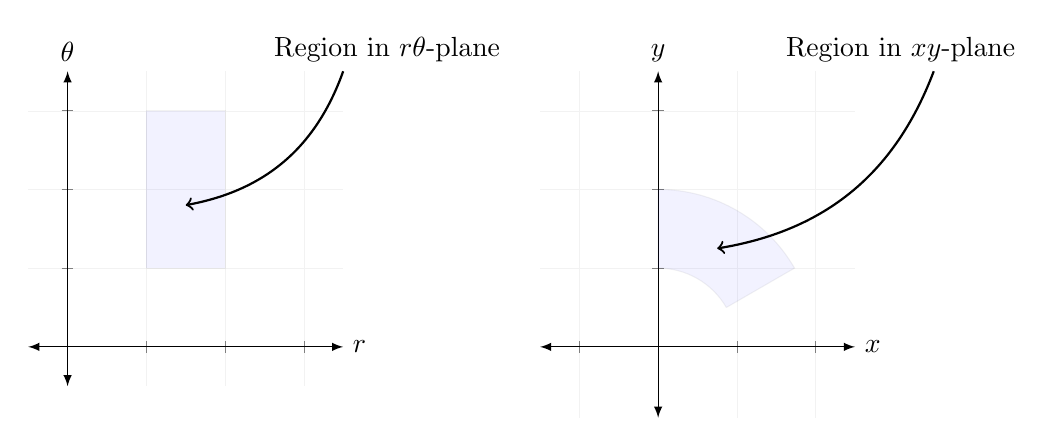
\begin{tikzpicture}


		\begin{axis}[
			name=plot1,
		    anchor=origin,
		    disabledatascaling,
		    xmin=-0,xmax=3,
		    ymin=-0,ymax=3,
		    x=1cm,y=1cm,
		    grid=both,
		    grid style={line width=.1pt, draw=gray!10},
		    %major grid style={line width=.2pt,draw=gray!50},
		    axis lines=middle,
		    minor tick num=0,
		    enlargelimits={abs=0.5},
		    axis line style={latex-latex},
			xticklabels={,,},
			yticklabels={,,},
			xlabel={$r$},
			ylabel={$\theta$},
		    xlabel style={at={(ticklabel* cs:1)},anchor=west},
		    ylabel style={at={(ticklabel* cs:1)},anchor=south}
		]

	\draw[fill=blue,opacity=0.05] (1,1) rectangle (2,3);	

	

		\end{axis}

		\draw[] (2.5,3.5) node[above right] {Region in $r\theta$-plane};
		\path[thick] (3.5,3.5) edge[bend left, ->] node[] {} (1.5,1.8);


		\begin{axis}[
			%at=(plot1.east),
			at={(7.5,0)},
		    anchor=origin,
		    disabledatascaling,
		    xmin=-1,xmax=2,
		    ymin=-0.4,ymax=3,
		    x=1cm,y=1cm,
		    grid=both,
		    grid style={line width=.1pt, draw=gray!10},
		    %major grid style={line width=.2pt,draw=gray!50},
		    axis lines=middle,
		    minor tick num=0,
		    enlargelimits={abs=0.5},
		    axis line style={latex-latex},
			xticklabels={,,},
			yticklabels={,,},
			xlabel={$x$},
			ylabel={$y$},
		    xlabel style={at={(ticklabel* cs:1)},anchor=west},
		    ylabel style={at={(ticklabel* cs:1)},anchor=south}
		]

	\draw[fill=blue,opacity=0.05] (30:1) -- (30:2) arc (30:90:2) -- (90:1) arc (90:30:1) node (pp) {};	
	
		\end{axis}	
		\draw[] (2.5+7.5,3.5) node[above right,xshift=-1cm] {Region in $xy$-plane};
		\path[thick] (3.5+7.5,3.5) edge[bend left, ->] node[] {} (.75+7.5,1.25);

	\end{tikzpicture}
\end{center}

While the graph of $r=\theta$ is a line in the $r\theta$-plane, it is a spiral in the $xy$-plane.

\begin{center}
	\begin{tikzpicture}


		\begin{axis}[
			name=plot1,
		    anchor=origin,
		    disabledatascaling,
		    xmin=-0,xmax=3,
		    ymin=-0,ymax=3,
		    x=1cm,y=1cm,
		    grid=both,
		    grid style={line width=.1pt, draw=gray!10},
		    %major grid style={line width=.2pt,draw=gray!50},
		    axis lines=middle,
		    minor tick num=0,
		    enlargelimits={abs=0.5},
		    axis line style={latex-latex},
			xticklabels={,,},
			yticklabels={,,},
			xlabel={$r$},
			ylabel={$\theta$},
		    xlabel style={at={(ticklabel* cs:1)},anchor=west},
		    ylabel style={at={(ticklabel* cs:1)},anchor=south}
		]

			\addplot[mypink, thick] {x};
		\end{axis}

		\begin{axis}[
			%at=(plot1.east),
			at={(7.5,0)},
		    anchor=origin,
		    disabledatascaling,
		    xmin=-2,xmax=2.2,
		    ymin=-2,ymax=3,
		    x=1cm,y=1cm,
		    grid=both,
		    grid style={line width=.1pt, draw=gray!10},
		    %major grid style={line width=.2pt,draw=gray!50},
		    axis lines=middle,
		    minor tick num=0,
		    enlargelimits={abs=0.5},
		    axis line style={latex-latex},
			xticklabels={,,},
			yticklabels={,,},
			xlabel={$x$},
			ylabel={$y$},
		    xlabel style={at={(ticklabel* cs:1)},anchor=west},
		    ylabel style={at={(ticklabel* cs:1)},anchor=south}
		]

	\addplot[mypink, thick, domain=0:3, samples=100,smooth] ({x*cos(deg(x)*5)},{x*sin(deg(x)*5)});
	
		\end{axis}	

	\end{tikzpicture}
\end{center}

Despite this discussion, expect coordinate systems to occasionally be confusing.  Still,
their usefulness in applications outweighs the inconvenience of being confused.  We will examine
a couple more of the most popular non-rectangular coordinate systems.

\subsection{Cylindrical Coordinates}
Cylindrical coordinates\index{cylindrical coordinates} is a coordinate system for $\R^3$
that arises as a straightforward extension of polar coordinates.  Every point in $\R^3$ is
described by three numbers denoted by $r$, $\theta$, and $z$.

Recall that $\R^3$ can be described as $\R^2\times\R$.  That is, any point in $\R^3$ can be described
as a point in $\R^2$ coupled with a ``$z$-height.''  Cylindrical coordinates are obtained by
writing points in $\R^2$ in polar coordinates and then adding a $z$ component.

\begin{center}
	\tdplotsetmaincoords{60}{110}

	\pgfmathsetmacro{\rvec}{.8}
	\pgfmathsetmacro{\thetavec}{30}
	\pgfmathsetmacro{\phivec}{60}

	%start tikz picture, and use the tdplot_main_coords style to implement the display 
	%coordinate transformation provided by 3dplot
	\begin{tikzpicture}[scale=5,tdplot_main_coords]

	%set up some coordinates 
	%-----------------------
	\coordinate (O) at (0,0,0);

	%determine a coordinate (P) using (r,\theta,\phi) coordinates.  This command
	%also determines (Pxy), (Pxz), and (Pyz): the xy-, xz-, and yz-projections
	%of the point (P).
	%syntax: \tdplotsetcoord{Coordinate name without parentheses}{r}{\theta}{\phi}
	\tdplotsetcoord{P}{\rvec}{\thetavec}{\phivec}

	%draw figure contents
	%--------------------

	%draw the main coordinate system axes
	\draw[thick,->] (0,0,0) -- (1,0,0) node[anchor=north east]{$x$};
	\draw[thick,->] (0,0,0) -- (0,1,0) node[anchor=north west]{$y$};
	\draw[thick,->] (0,0,0) -- (0,0,1) node[anchor=south]{$z$};

	%draw a vector from origin to point (P) 
	\draw[-latex,color=mypink, thick] (O) -- (P);

	%draw projection on xy plane, and a connecting line
	\draw[dashed, color=lightgray, ->] (O) -- (Pxy) node[right, black] {$r$};
	\draw[dashed, color=lightgray,->] (Pxy) -- (P) node[midway, above right, black,yshift=.2cm] {$z$};

	%draw the angle \phi, and label it
	%syntax: \tdplotdrawarc[coordinate frame, draw options]{center point}{r}{angle}{label options}{label}
	\tdplotdrawarc{(O)}{0.2}{0}{\phivec}{anchor=north}{$\theta$};
	\tdplotdrawarc[dashed,lightgray]{(O)}{0.4}{0}{360}{anchor=north}{};

	\draw[fill=black] (P) circle (.4pt) node[right] {$(r,\theta, z)$};

	\end{tikzpicture}
\end{center}

They are related to rectangular coordinates by the formulas
\[
	x=r\cos\theta\qquad
	y=r\sin\theta\qquad
	z=z
\]
where $(r,\theta,z)$ represents a point in cylindrical coordinates and $(x,y,z)$ is the same point in rectangular
coordinates.



\begin{example}  $r = a$ describes an (infinite) cylinder
of radius $a$ centered on the $z$-axis.  If we let $a$ vary, we
obtain an infinite family of concentric cylinders.  We can treat
the case $a = 0$ (the $z$-axis) as a degenerate cylinder of
radius 0.

	\begin{center}
	\begin{tikzpicture}
	    \begin{axis}[grid=major,view={20}{20},z buffer=sort,
		    %shader=faceted interp,
		    %patch type=biquadratic,
		    colormap/copper,
		    %width=12cm,
		    %scale mode=scale uniformly,
		    %zmin=-5,zmax=5,xmin=-10,xmax=10,ymin=-10,ymax=10,
		    xticklabels={,,}, yticklabels={,,}, zticklabels={,,},
		    %xtick={-10,-5,...,10}, ytick={-10,-5,...,10}
		    ]
		    \addplot3[surf, colormap/viridis,
		    z buffer=sort,samples=20,
			variable=\u, variable y=\v,
			domain=-180:180, y domain=-2:3]
			({2*cos(u)}, {2*sin(u)}, {v});
	    \end{axis}
	  \end{tikzpicture}
	\end{center}
\end{example}

\begin{example}$\theta = \alpha$ describes a \emph{half
plane} making angle $\alpha$ with the positive $xz$-plane.
In this half plane, $r$ can assume any non-negative
value and $z$ can assume any value.

	\begin{center}
		\tdplotsetmaincoords{60}{110}

		\pgfmathsetmacro{\rvec}{.5}
		\pgfmathsetmacro{\thetavec}{30}
		\pgfmathsetmacro{\phivec}{60}

		%start tikz picture, and use the tdplot_main_coords style to implement the display 
		%coordinate transformation provided by 3dplot
		\begin{tikzpicture}[scale=3,tdplot_main_coords]

		%set up some coordinates 
		%-----------------------
		\coordinate (O) at (0,0,0);

		%determine a coordinate (P) using (r,\theta,\phi) coordinates.  This command
		%also determines (Pxy), (Pxz), and (Pyz): the xy-, xz-, and yz-projections
		%of the point (P).
		%syntax: \tdplotsetcoord{Coordinate name without parentheses}{r}{\theta}{\phi}
		\tdplotsetcoord{P}{\rvec}{\thetavec}{\phivec}
		\tdplotsetcoord{A}{.9}{0}{60}
		\tdplotsetcoord{D}{.64}{180}{60}
		\tdplotsetcoord{B}{1.35}{45}{60}
		\tdplotsetcoord{C}{1.17}{125}{60}

		%draw figure contents
		%--------------------

		%draw the main coordinate system axes
		\draw[thick,->] (0,0,0) -- (1,0,0) node[anchor=north east]{$x$};
		\draw[thick,->] (0,0,0) -- (0,1,0) node[anchor=north west]{$y$};
		\draw[thick,->] (0,0,0) -- (0,0,1) node[anchor=south]{$z$};

		%draw a vector from origin to point (P) 

		\draw[fill=myorange, opacity=.4] (A) -- (B) -- (C) -- (D) --cycle;

		%draw projection on xy plane, and a connecting line
		\draw[dashed, color=lightgray] (O) -- (Bxy);


		%draw the angle \phi, and label it
		%syntax: \tdplotdrawarc[coordinate frame, draw options]{center point}{r}{angle}{label options}{label}
		\tdplotdrawarc{(O)}{0.2}{0}{\phivec}{anchor=north}{$\alpha$};


		\draw[fill=black] (P) node[right] {$\theta=\alpha$};

		\end{tikzpicture}
	\end{center}
\end{example}
\begin{example}  $z = mr$  describes an (infinite)
  cone centered
on the $z$-axis with vertex at the origin.  For a fixed value
of $\theta$, we obtain a ray in this cone which starts at
the origin and extends to infinity.  This ray makes angle
$\arctan m$ with the $z$-axis, and if we let $\theta$
vary, the ray rotates around the $z$-axis generating the
cone.  Note also that if $m > 0$, the angle with the $z$-axis
is acute and the cone lies above the $xy$-plane.  If
$m < 0$, the angle is obtuse, and the cone lies below the
$xy$-plane.  The case $m = 0$ yields the $x,y$-plane
($z = 0$) which may be considered a special `cone'.

Note that in rectangular coordinates,  $z = mr$ becomes
$z = m\sqrt{x^2 + y^2}$.

	\begin{center}
	\begin{tikzpicture}
	    \begin{axis}[grid=major,view={20}{20},z buffer=sort,
		    %shader=faceted interp,
		    %patch type=biquadratic,
		    colormap/copper,
		    %width=12cm,
		    %scale mode=scale uniformly,
		    %zmin=-5,zmax=5,xmin=-10,xmax=10,ymin=-10,ymax=10,
		    xticklabels={,,}, yticklabels={,,}, zticklabels={,,},
		    %xtick={-10,-5,...,10}, ytick={-10,-5,...,10}
		    ]
		    \addplot3[surf, 
		    z buffer=sort,samples=20,
			variable=\u, variable y=\v,
			domain=-180:180, y domain=0:3]
			({2*v*cos(u)}, {2*v*sin(u)}, {v});
	    \end{axis}
	  \end{tikzpicture}
	\end{center}
\end{example}

\begin{example}  $r^2 + z^2 = a^2$ describes a sphere
of radius $a$ centered at the origin.  The easiest way to
see this is to put $r^2 = x^2 + y^2$ whence the equation
becomes $x^2 + y^2 + z^2 = a^2$.  The top hemisphere of the
sphere would be described by $z = \sqrt{a^2 - r^2}$
and the bottom hemisphere by
 $z = -\sqrt{a^2 - r^2}$.
\end{example}


\subsection{Spherical Coordinates}

Cylindrical coordinates are one way to generalize polar coordinates
to $\R^3$, but there is another way that is more useful for
problems with spherical symmetry. 
\emph{Spherical
coordinates}
\index{spherical coordinates}
\index{coordinates, spherical}
are denoted with the variables $\rho$, $\phi$, and $\theta$.

A point $P$ in space is defined by the coordinates $(\rho,\theta,\phi)$ as follows.   
The coordinate $\rho$ gives the distance
$\norm{\overrightarrow{OP}}$ of the point
to the origin.  It is always non-negative, and it should be
distinguished from the cylindrical coordinate $r$ which is the
distance from the $z$-axis.  The coordinate $\phi$ gives
the \emph{azimuthal angle}\index{azimuthal angle}, which
is the angle of declination between $\overrightarrow{OP}$ and the positive $z$-axis.
We will assume $\phi\in[0,\pi]$.  Finally, the coordinate $\theta$
denotes the \emph{longitudinal angle}\index{longitudinal angle},
and is the same as the $\theta$ from cylindrical coordinates.
Again, we assume $\theta\in[0,2\pi)$.

\begin{center}
	\tdplotsetmaincoords{60}{110}

	\pgfmathsetmacro{\rvec}{.8}
	\pgfmathsetmacro{\thetavec}{30}
	\pgfmathsetmacro{\phivec}{60}

	%start tikz picture, and use the tdplot_main_coords style to implement the display 
	%coordinate transformation provided by 3dplot
	\begin{tikzpicture}[scale=5,tdplot_main_coords]

	%set up some coordinates 
	%-----------------------
	\coordinate (O) at (0,0,0);

	%determine a coordinate (P) using (r,\theta,\phi) coordinates.  This command
	%also determines (Pxy), (Pxz), and (Pyz): the xy-, xz-, and yz-projections
	%of the point (P).
	%syntax: \tdplotsetcoord{Coordinate name without parentheses}{r}{\theta}{\phi}
	\tdplotsetcoord{P}{\rvec}{\thetavec}{\phivec}

	%draw figure contents
	%--------------------

	%draw the main coordinate system axes
	\draw[thick,->] (0,0,0) -- (1,0,0) node[anchor=north east]{$x$};
	\draw[thick,->] (0,0,0) -- (0,1,0) node[anchor=north west]{$y$};
	\draw[thick,->] (0,0,0) -- (0,0,1) node[anchor=south]{$z$};

	%draw a vector from origin to point (P) 
	\draw[-latex,color=mypink, thick] (O) -- (P);




	%draw the angle \phi, and label it
	%syntax: \tdplotdrawarc[coordinate frame, draw options]{center point}{r}{angle}{label options}{label}
	\tdplotdrawarc{(O)}{0.2}{0}{\phivec}{anchor=north}{$\theta$};

	%set the rotated coordinate system so the x'-y' plane lies within the
	%"theta plane" of the main coordinate system
	%syntax: \tdplotsetthetaplanecoords{\phi}
	\tdplotsetthetaplanecoords{\phivec}

	%draw theta arc and label, using rotated coordinate system
	\tdplotdrawarc[tdplot_rotated_coords]{(0,0,0)}{0.5}{0}{\thetavec}{anchor=south west}{$\phi$}

	%draw some dashed arcs, demonstrating direct arc drawing
	\draw[dashed,tdplot_rotated_coords,] (\rvec,0,0) arc (0:90:\rvec) node (RHO) {};
	\draw[dashed] (\rvec,0,0) arc (0:90:\rvec);

	%draw projection on xy plane, and a connecting line
	\draw[dashed, color=lightgray]  (Pxy) -- (P);
	\draw[dashed, color=lightgray]  (O) -- (RHO);

	\draw[fill=black] (P) circle (.4pt) node[right] {$(\rho,\theta, \phi)$};
\draw (RHO) node[below right] {$\rho$};

	\end{tikzpicture}
\end{center}

Note the reason we restrict $\phi$ to the interval $[0,\pi]$ (rather than
$[0,2\pi]$). Fix $\rho$
and $\theta$.   If $\phi = 0$,
the point is on the positive $z$-axis, and, as $\phi$ increases,
the point swings down toward the negative $z$-axis. However, it stays
in the half plane determined by that value of $\theta$.  For
$\phi = \pi$, the point is on the negative $z$-axis, but if we
allow $\phi$ to increase further, the point swings into the
\emph{opposite} half plane with longitudinal angle $\theta + \pi$.
Such points can be obtained just as well by swinging down from
the positive $z$-axis in the opposite half plane determined by
$\theta + \pi$.

The following relationships hold between spherical coordinates,
cylindrical coordinates, and rectangular coordinates. 
\begin{align*}
	r & = \rho \sin\phi \\
	z & = \rho \cos\phi \\
	\intertext{so}
	x &=  \rho \sin\phi \cos\theta \\
	y &=  \rho \sin\phi \sin\theta \\
	z & = \rho \cos\phi\\
	\intertext{and}
	\rho &= \sqrt{r^2 + z^2} = \sqrt{x^2 + y^2 + z^2} \\
	\tan\phi &= \frac rz\qquad\text{if } z \ne 0.
\end{align*}

It is important to note that unlike rectangular, polar, or cylindrical coordinates,
mathematicians and physicists use two different conventions for spherical coordinates.
We have introduced spherical coordinates in the order $(\rho,\theta,\phi)$.  This
paints spherical coordinates as an extension of polar coordinates in the $xy$-plane by
the addition of a third coordinate, $\phi$.  However, ordered this way, spherical
coordinates produce a \emph{left-handed} coordinate system.  Since physicists prefer
right-handed coordinate systems, they tend to use the order $(\rho,\phi,\theta)$ when
describing points in spherical coordinates\footnote{ Mathematics and physicists
differ in their conventions in several other regards.  Often times a force that is negative
to a physicist is positive to a mathematician and mathematicians tend to reverse the temperature
scale when doing thermodynamics.  All of the theorems come out the same, of course,
but it takes some interpretation to understand theorems from another field.}.  
We will primarily use the mathematical convention,
but when you read problems presented in spherical coordinates in other contexts, be
aware of what convention the author is using!


\begin{example}
$\rho = a$ describes a sphere of radius $a$ centered at the origin.
\end{example}

\begin{example}
$\phi = \alpha$ describes a cone making angle $\alpha$ with the
positive $z$-axis.  If $\phi<\pi/2$ the cone lies above the $xy$-plane;
	if $\phi>\pi/2$, the cone lies below the $xy$-plane; 
	and if $\phi=\pi/2$, the (degenerate) cone \emph{is} the $xy$-plane.
\end{example}

\begin{example}
$\theta = \beta$ describes a half plane starting from the $z$-axis
as before.
\end{example}

\begin{example}
$\rho = 2a\cos\phi$ describes a sphere of radius
$a$ centered at $(0,0,a)$.  You can see this by looking at
the half plane determined by fixing $\theta$.  In that half
plane, the locus is the \emph{semi-circle} with the given
radius and center.  If we then let $\theta$ vary, the effect is
to rotate the semi-circle about the $z$-axis and generate the
sphere

	\begin{center}
		\tdplotsetmaincoords{60}{110}

		\pgfmathsetmacro{\rvec}{.8}
		\pgfmathsetmacro{\thetavec}{30}
		\pgfmathsetmacro{\phivec}{60}

		%start tikz picture, and use the tdplot_main_coords style to implement the display 
		%coordinate transformation provided by 3dplot
		\begin{tikzpicture}[scale=3,tdplot_main_coords]

		%set up some coordinates 
		%-----------------------
		\coordinate (O) at (0,0,0);

		%determine a coordinate (P) using (r,\theta,\phi) coordinates.  This command
		%also determines (Pxy), (Pxz), and (Pyz): the xy-, xz-, and yz-projections
		%of the point (P).
		%syntax: \tdplotsetcoord{Coordinate name without parentheses}{r}{\theta}{\phi}
		\tdplotsetcoord{P}{\rvec}{\thetavec}{\phivec}

		%draw figure contents
		%--------------------

		%draw the main coordinate system axes
		\draw[thick,->] (0,0,0) -- (1,0,0) node[anchor=north east]{$x$};
		\draw[thick,->] (0,0,0) -- (0,1,0) node[anchor=north west]{$y$};
		\draw[thick,->] (0,0,0) -- (0,0,1) node[anchor=south]{$z$};

		%draw the angle \phi, and label it
		%syntax: \tdplotdrawarc[coordinate frame, draw options]{center point}{r}{angle}{label options}{label}
		\tdplotdrawarc{(O)}{0.2}{0}{\phivec}{anchor=north}{$\theta$};

		%set the rotated coordinate system so the x'-y' plane lies within the
		%"theta plane" of the main coordinate system
		%syntax: \tdplotsetthetaplanecoords{\phi}
		\tdplotsetthetaplanecoords{\phivec}
		
		%draw theta arc and label, using rotated coordinate system
		%\tdplotdrawarc[tdplot_rotated_coords]{(0,0,0)}{0.5}{0}{\thetavec}{anchor=south west}{$\phi$}
		
		\draw[tdplot_rotated_coords] (0,0,0) arc (0:-90:-.4) node (X) {};
		\draw[tdplot_rotated_coords, mypink, ultra thick] (0,0,0) arc (0:360:-.4);


		%draw projection on xy plane, and a connecting line
		\draw[dashed, color=lightgray]  (Pxy) -- (X);
		\draw[dashed, color=lightgray]  (O) -- (Pxy);

		\tdplotsetthetaplanecoords{30}
		\draw[tdplot_rotated_coords, myorange, ultra thin] (0,0,0) arc (0:360:-.4);
		\tdplotsetthetaplanecoords{90}
		\draw[tdplot_rotated_coords, myorange, ultra thin] (0,0,0) arc (0:360:-.4);
		\tdplotsetthetaplanecoords{120}
		\draw[tdplot_rotated_coords, myorange, ultra thin] (0,0,0) arc (0:360:-.4);
		\tdplotsetthetaplanecoords{150}
		\draw[tdplot_rotated_coords, myorange, ultra thin] (0,0,0) arc (0:360:-.4);
		\tdplotsetthetaplanecoords{180}
		\draw[tdplot_rotated_coords, myorange, ultra thin] (0,0,0) arc (0:360:-.4);
		\end{tikzpicture}
	\end{center}
\end{example}

If we fix $\rho = a$, we obtain a sphere of radius $a$.
Then $(\phi, \theta)$ specify the position of a point on
that sphere.  

For $\theta = $ constant, we obtain the semi-circle
which is the intersection of the half plane for that $\theta$
with the sphere.  That circle is called a {\it meridian of
longitude}.  This is exactly the concept of longitude used to
\index{meridian of longitude}
\index{longitude}
measure position on the surface of the Earth, except that we
use radians instead of degrees.  Earth's longitude is usually
measured in degrees east or west of the Greenwich Meridian.
That corresponds in our case to the positive and negative
directions from the 0-meridian.  

\begin{center}
	\pgfplotsset{compat=1.9}
	%\usetikzlibrary{arrows.meta}

	\begin{tikzpicture}
	\def\tilt{45}
	\def\azimuth{30}
	\begin{axis}[%
	axis equal,
	width=14cm,
	height=14cm,
	hide axis,
	enlargelimits=0.3,
	view/h=\tilt,
	view/v=\azimuth,
	scale uniformly strategy=units only,
	colormap={bluewhite}{color=(blue) color=(white)},   
	]
	\coordinate (X) at (axis cs: 1,0,0);
	\coordinate (-X) at (axis cs: -1,0,0);
	\coordinate (Y) at (axis cs: 0,1,0);
	\coordinate (-Y) at (axis cs: 0,-1,0);
	\coordinate (Z) at (axis cs: 0,0,1);
	\coordinate (-Z) at (axis cs: 0,0,-1);
	\filldraw[ball color=white,draw=none] (axis cs: 0,0,0) circle (2.47cm);
	    \pgfplotsinvokeforeach {-80,-60,...,80}{
		\pgfplotsextra{ 
		    \pgfmathsetmacro\sinVis{sin(#1)/cos(#1)*sin(30)/cos(30)}
		    % angle of "visibility"
		    \pgfmathsetmacro\angVis{asin(min(1,max(\sinVis,-1)))}
		    \coordinate (X) at (axis cs: {cos(#1)},0,{sin(#1)});
		    \draw [densely dashed, lightgray] (X) arc (0:360:{100*cos(#1)});
		} }


	\foreach \a in {0}
	{ \pgfmathsetmacro{\Bound}{-60*cos(\a+45)}
	    \addplot3[domain=\Bound:90, samples=45,samples y=0, mypink, ultra thick] ({cos(\a)*cos(x)},{sin(\a)*cos(x)},{sin(x)});
	    \addplot3[domain=-90:\Bound, samples=45,samples y=0, densely dashed, mypink, ultra thick] ({cos(\a)*cos(x)},{sin(\a)*cos(x)},{sin(x)});
	}

	\foreach \a in {180}
	{ \pgfmathsetmacro{\Bound}{-60*cos(\a+45)}
	    \addplot3[domain=\Bound:90, samples=45,samples y=0] ({cos(\a)*cos(x)},{sin(\a)*cos(x)},{sin(x)});
	    \addplot3[domain=-90:\Bound, samples=45,samples y=0, densely dashed] ({cos(\a)*cos(x)},{sin(\a)*cos(x)},{sin(x)});
	}

	\draw (4.1cm,2cm) node {0-meridian};

	\end{axis}  
	\end{tikzpicture}  
\end{center}


For $\phi = $ constant, we obtain the circle which is the
intersection of the cone for that $\phi$ with the sphere.
Such circles are called {\it circles of latitude}.
\index{circle of latitude}
\index{latitude}
The coordinate $\phi$ is related to the notion of latitude on the surface
of the Earth, except that the latter is an angle
in degrees north or south of the \emph{equatorial plane}.  The
spherical coordinate $\phi$ is sometimes called \emph{co-latitude},
and we have $\phi = \pi/2 - \lambda$, where $\lambda$ is the latitude
measures from the equatorial plane (assuming both $\lambda$ and $\phi$ are
measured in radians).
The unique point with $\phi = 0$ is called the
\emph{north pole}, that with $\phi = \pi$ is called the
\emph{south pole}, and at the  poles $\theta$ is not well defined.


\subsection{Coordinate Systems from Parameterizations}
We've looked at several important coordinate systems for $\R^2$ and $\R^3$,
but any parameterization of $\R^2$ or $\R^3$ gives rise to a coordinate system.

Consider $\vec p:\R^2\to\R^2$ given by $\vec p(a,b)=(a-b,a+b)$.  

\begin{exercise}
	Show that $\vec p:\R^2\to\R^2$ given by $\vec p(a,b)=(a-b,a+b)$ is
	a parameterization.  That is, that it is a continuous 
	one-to-one and onto function.
\end{exercise}

Geometrically, we can view $\vec p$ as taking the plane, rotating it by $45^\circ$,
and then
stretching it uniformly in all directions by a factor of $\sqrt{2}$.

Alternatively, we can imagine that $\vec p$ describes how to take points described
in ``$ab$-coordinates'' and rewrite them in rectangular coordinates.  Call this new coordinate
system $\mathcal A$. We then get that
$\mathcal A$ coordinates relate to rectangular coordinates by
\[
	x=a-b\qquad\text{and}\qquad y=a+b.
\]
Drawing the lines $a=0$ and $b=0$ we see that $\mathcal A$ coordinates are very similar to
rectangular coordinates but with rotated and scaled axes.

\begin{center}
	\begin{tikzpicture}
		\begin{axis}[
			name=plot1,
		    anchor=origin,
		    disabledatascaling,
		    xmin=-1,xmax=5,
		    ymin=-1,ymax=3,
		    x=1cm,y=1cm,
		    grid=both,
		    grid style={line width=.1pt, draw=gray!10},
		    %major grid style={line width=.2pt,draw=gray!50},
		    axis lines=middle,
		    minor tick num=0,
		    enlargelimits={abs=0.5},
		    axis line style={latex-latex},
			xticklabels={,,},
			yticklabels={,,},
			xlabel={$a$},
			ylabel={$b$},
		    xlabel style={at={(ticklabel* cs:1)},anchor=west},
		    ylabel style={at={(ticklabel* cs:1)},anchor=south}
		]

	\foreach \i in {-1,...,5} {
		\addplot[color=myorange, dashed, thick, domain=-3:5] ({\i},{x});
		\addplot[color=blue, dashed, thick, domain=-3:6] ({x},{\i});
%		\addplot[color=blue, dashed] ({1}{x});
}
		\draw[fill] (2,-1) circle (1.5pt) node (A) {};
		\end{axis}



		\path[thick] (3.5,3.5) node[above] {$(a,b)=(2,-1)$} edge[bend left, ->] node[] {} (A);


		\begin{axis}[
			%at=(plot1.east),
			at={(7.5,0)},
		    anchor=origin,
		    disabledatascaling,
		    xmin=-1,xmax=5,
		    ymin=-1.4,ymax=3,
		    x=1cm,y=1cm,
		    grid=both,
		    grid style={line width=.1pt, draw=gray!10},
		    %major grid style={line width=.2pt,draw=gray!50},
		    axis lines=middle,
		    minor tick num=0,
		    enlargelimits={abs=0.5},
		    axis line style={latex-latex},
			xticklabels={,,},
			yticklabels={,,},
			xlabel={$x$},
			ylabel={$y$},
		    xlabel style={at={(ticklabel* cs:1)},anchor=west},
		    ylabel style={at={(ticklabel* cs:1)},anchor=south}
		]

	\foreach \i in {-5,...,5} {
		\addplot[color=myorange, dashed, thick, domain=-3:5] ({\i-x},{x+\i});
		\addplot[color=blue, dashed, thick, domain=-3:6] ({x-\i},{\i+x});
}

		\draw[fill] (3,1) circle (1.5pt) node (B) {};	
		\end{axis}	

		\path[thick] (3.5+7.5,3.5) node[above] {$(x,y)=\vec p(2,-1)$} edge[bend left, ->] node[] {} (B);

	\end{tikzpicture}
\end{center}

There might be good reason to use $\mathcal A$ coordinates, depending on your application.
For example, suppose you were working on a construction project and you are using rectangular
coordinates $(x,y)$ to represent the position north and east from the origin of your construction
lot.  If you're building a diagonal building, it might be nicer to describe locations in your building
using $\mathcal A$ coordinates.

\bigskip

Now, we might be tempted to propose that all coordinate systems come from parameterizations,
and this is \emph{almost} true.  However, coordinate systems like polar, cylindrical, and spherical
all have \emph{singularities}.  That is, there are points in space that are not uniquely
describable in those coordinate systems.  Thus, if we consider, for example, the function
$\vec p:\R^2\to\R^2$ which converts polar coordinates to rectangular coordinates, it isn't a true
parameterization because it isn't one-to-one at the origin.  We won't let this detail bother us---polar,
cylindrical, and spherical coordinates are still useful and they \emph{almost} come from parameterizations.
Occasionally we will even slip up and proclaim that $\R^2$ is parameterized by polar coordinates
or that $\R^3$ is parameterized by spherical coordinates\footnote{
	To a novice mathematician, it can be hard to discern the 
	patterns in what determines where a professional mathematician allows
	herself to be sloppy and where she maintains excruciating logical precision.
	Rest assured, after enough mistakes, one learns where one needs to tread carefully
	and where one can be more lax.
}.

\begin{exercises}
\end{exercises}
